% IEEE Conference Template -- Data Mining 2026 Final Project, Team 4
% Multi-Faceted Customer Intelligence for E-commerce on Online Retail II
%
% NOTE: This is the TEMPLATE. Do not edit metric numbers here by hand --
% edit prose only. `overleaf/main.tex` is GENERATED from this file by
% `python -m src.report_renderer`, which fills the metric placeholders from the current
% pipeline artifacts. Re-render after any pipeline re-run.
%
% Upload the generated main.tex + figures (and references.bib) to a fresh
% Overleaf project based on the IEEE Conference template:
%   https://www.overleaf.com/latex/templates/ieee-conference-template/grfzhhncsfqn

\documentclass[conference]{IEEEtran}
\IEEEoverridecommandlockouts
\usepackage{cite}
\usepackage{amsmath,amssymb,amsfonts}
\usepackage{algorithmic}
\usepackage{graphicx}
\usepackage{textcomp}
\usepackage{xcolor}
\usepackage{booktabs}
\usepackage{url}
\usepackage{hyperref}
\def\BibTeX{{\rm B\kern-.05em{\sc i\kern-.025em b}\kern-.08em
    T\kern-.1667em\lower.7ex\hbox{E}\kern-.125emX}}

\begin{document}

\title{Multi-Faceted Customer Intelligence for E-commerce:\\
An End-to-End Data Mining Pipeline on Online Retail II}

\author{
\IEEEauthorblockN{Nguyen Minh Cuong}
\IEEEauthorblockA{22520177\\
University of Information Technology\\
VNU-HCM, Vietnam}
\and
\IEEEauthorblockN{Vo Thanh Danh}
\IEEEauthorblockA{22520201\\
University of Information Technology\\
VNU-HCM, Vietnam}
\and
\IEEEauthorblockN{Nguyen Vinh Dat}
\IEEEauthorblockA{22520228\\
University of Information Technology\\
VNU-HCM, Vietnam}
\and
\IEEEauthorblockN{Nguyen Huu Dinh}
\IEEEauthorblockA{22520251\\
University of Information Technology\\
VNU-HCM, Vietnam}
}

\maketitle

\begin{abstract}
Retaining existing customers is dramatically cheaper than acquiring new ones, yet most e-commerce platforms still treat customer segmentation, churn prediction, and market-basket analysis as independent problems. We present an end-to-end data mining pipeline on the UCI Online Retail II dataset (1{,}067{,}371 raw transactions, {{n_clean_rows}} after cleaning, {{n_customers_total}} unique customers, 2009--2011) that unifies all three tasks and adds a deep-learning extension. Customers are first segmented with K-means, DBSCAN, and AGNES on log-transformed RFM features; K-means with $k=2$ achieves the best Silhouette of {{clustering_silhouette}}, separating a dormant majority (54\%, mean Recency 317 days) from an active high-value minority (46\%, mean spend \pounds 5{,}206). A 90-day churn label is then predicted by six classical algorithms and an MLP under a strict leakage-safe protocol---all supervised features are computed before the cutoff and every transformer is fit on training folds only; {{classification_best_model}} leads with AUC {{classification_best_auc}} and the MLP reaches {{classification_mlp_auc}}, both well above majority-class ({{majority_auc}}) and recency-only ({{recency_auc}}) baselines. Apriori and FP-Growth surface {{association_n_rules}} product association rules (top lift {{top_rule_lift}} on the Regency teacup pair); FP-Growth runs $1.5\times$ faster than Apriori at identical parameters. An autoencoder flags the top 5\% of customers by reconstruction error as behavioural anomalies. The cross-task synthesis reveals a {{churn_gap_points}}-percentage-point churn gap between the two segments (90\% vs 23\%) and shows that the loyal segment buys in color-coordinated pairs (lift 5.3--7.4), producing actionable segment-aware retention recommendations no single model could surface alone. All experiments are reproducible from a public repository.
\end{abstract}

\begin{IEEEkeywords}
data mining, customer segmentation, churn prediction, association rule mining, deep learning, autoencoder, SHAP, RFM
\end{IEEEkeywords}

% ========================================================================
\section{Introduction}
% ========================================================================
E-commerce retailers face three intertwined questions about their customer base: \emph{who they are}, \emph{who is about to leave}, and \emph{what they tend to buy together}. Solving any of these in isolation misses the cross-task synergies that drive real business actions: targeted retention is most effective when the offer matches the segment's basket signature, and anomalous behaviour is most actionable when localised within a coherent segment.

In this work we build a single coherent pipeline on the UCI Online Retail II dataset that addresses all three questions and demonstrates how their outputs reinforce one another. Our contributions are:
\begin{itemize}
  \item A reproducible end-to-end pipeline covering preprocessing, RFM engineering, three clustering algorithms, six classical churn classifiers, an MLP, market-basket mining via Apriori and FP-Growth, and an autoencoder for anomaly detection.
  \item A cross-task synthesis that maps churn rate, anomalous behaviour, and basket patterns onto the segmentation, surfacing segment-specific retention recommendations.
  \item An empirical comparison of all algorithm families under a unified evaluation framework (held-out test, 5-fold cross-validation, multiple internal cluster-validity indices, runtime).
\end{itemize}

% ========================================================================
\section{Related Work}
% ========================================================================
\textbf{RFM segmentation.} The Recency--Frequency--Monetary framework introduced by Hughes~\cite{hughes1994} remains a strong baseline for customer-value scoring and is the conventional input to clustering. \textbf{Clustering.} K-means~\cite{macqueen1967}, DBSCAN~\cite{ester1996} and Ward's agglomerative method~\cite{ward1963} cover partitional, density-based, and hierarchical regimes; the comparative study of Steinbach et al.~\cite{steinbach2000} provides validation methodology we follow. \textbf{Churn prediction.} Recent surveys~\cite{vafeiadis2015,ahmad2019,wagh2024} show tree ensembles and gradient boosting routinely top classical classifiers for tabular churn. \textbf{Class imbalance.} SMOTE~\cite{chawla2002} remains the standard oversampling approach for $\le$30\% positive-class problems. \textbf{Association rules.} Apriori~\cite{agrawal1994} and FP-Growth~\cite{han2000} dominate frequent-pattern mining; Borgelt~\cite{borgelt2012} surveys their efficiency trade-offs. \textbf{Explainability.} SHAP values~\cite{lundberg2017} provide model-agnostic local and global feature attributions. \textbf{Anomaly detection with autoencoders.} Reconstruction-error thresholding on autoencoders is a well-established unsupervised anomaly detector~\cite{sakurada2014,zhou2017}.

% ========================================================================
\section{Methodology}
% ========================================================================
Figure~\ref{fig:arch} gives the end-to-end architecture; the subsections below describe each stage in turn.

\begin{figure*}[t]
  \centering
  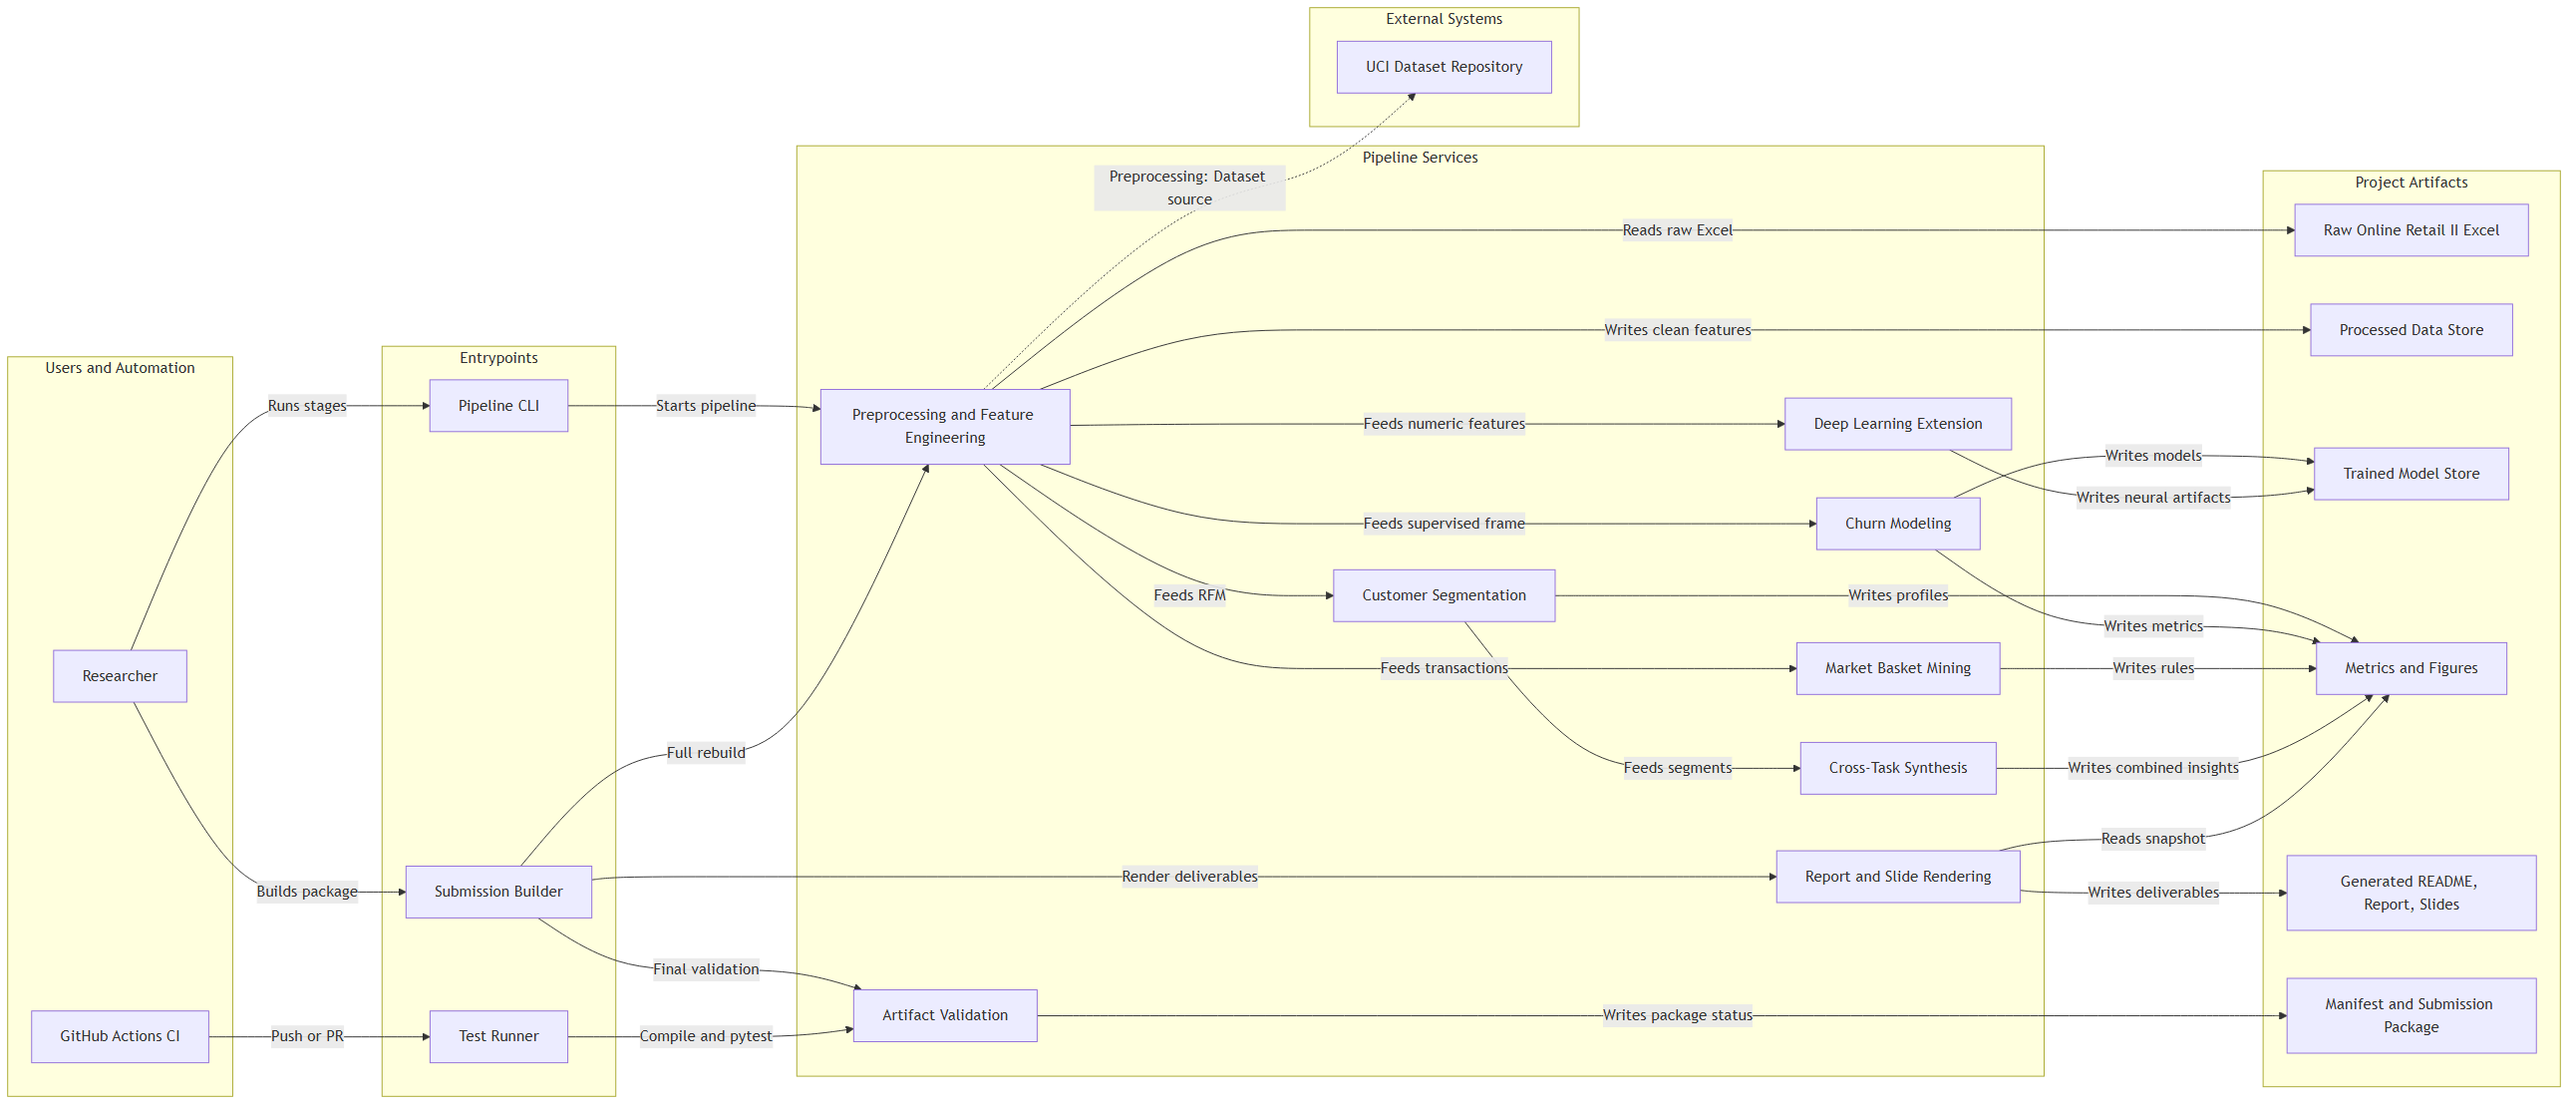
\includegraphics[width=0.96\textwidth]{figures/00_architecture.png}
  \caption{End-to-end system architecture: users/automation $\to$ entry points $\to$ pipeline services (preprocessing, segmentation, churn modelling, market-basket mining, deep learning, cross-task synthesis, report/slide rendering, validation) $\to$ artifact stores. Every metric reported in this paper is regenerated by this pipeline and recorded in \texttt{manifest.json}.}
  \label{fig:arch}
\end{figure*}

\subsection{Dataset and preprocessing}
We use Online Retail II from the UCI repository~\cite{uci_retail2}: 1{,}067{,}371 invoice-line records spanning 2009-12-01 to 2011-12-09 across 41 countries (92\% UK). Each record has exactly eight raw fields---\texttt{Invoice}, \texttt{StockCode}, \texttt{Description}, \texttt{Quantity}, \texttt{InvoiceDate}, \texttt{Price}, \texttt{CustomerID}, \texttt{Country}---all transaction-level: the dataset carries \emph{no} customer attributes (no name, contact details, or demographics) beyond the \texttt{CustomerID} key. Every cleaning step is therefore principled rather than arbitrary. (i)~Rows with a missing \texttt{CustomerID}---the only customer key in the schema---cannot be attributed to any customer and are unusable for the customer-level RFM, segmentation and churn tasks; importantly, such a row holds no other recoverable customer information, so nothing usable is lost. (ii)~Cancellation invoices (prefix \emph{C}) and non-positive \texttt{Quantity}/\texttt{Price} are returns, write-offs or data-entry artefacts rather than genuine purchases, and would distort spend and basket statistics. (iii)~\texttt{Quantity} and \texttt{Price} are winsorised at the 1\%/99\% quantiles so that a few extreme bulk lines do not dominate the distances and means used downstream. We then derive \texttt{TotalAmount = Quantity * Price}. For full-history segmentation we compute Recency (days from last purchase to snapshot 2011-12-10), Frequency (unique invoices), and Monetary (sum of TotalAmount), plus \texttt{avg\_basket\_value}, \texttt{avg\_basket\_size}, \texttt{unique\_products}, and \texttt{DominantCountry}. For the supervised churn task the same features are recomputed using only transactions strictly before the {{churn_cutoff}} cutoff (see below).

\subsection{Customer segmentation (Clustering)}
Frequency and Monetary are right-skewed and are log-transformed; all three RFM features are then standardised. We compare:
\begin{itemize}
  \item \textbf{K-means} with $k$ chosen by joint elbow + silhouette sweep over $k=2..10$.
  \item \textbf{DBSCAN} with $\varepsilon$ chosen from the elbow of the 4-NN distance plot~\cite{ester1996} and \texttt{min\_samples}=5.
  \item \textbf{AGNES} (Ward linkage) cut at the same $k$ chosen for K-means; dendrogram inspection confirms the cut.
\end{itemize}
Internal validation uses Silhouette, Davies--Bouldin, and Calinski--Harabasz indices, and we additionally re-run K-means over 10 seeds to confirm the silhouette and cluster sizes are stable. Two-dimensional visualisations use PCA and t-SNE.

\subsection{Churn prediction (Classification)}
A customer is labelled \emph{churned} if active before the {{churn_cutoff}} cutoff and absent during the {{churn_window_days}}-day window thereafter. Crucially, to avoid target leakage the feature matrix is built only from transactions \emph{before} the cutoff (with the snapshot set to the cutoff), and all encoding---log-scaling and a rare-folded one-hot of \texttt{DominantCountry}---is performed inside the cross-validation pipeline, so it is fit on training folds only. We train Logistic Regression, Decision Tree, Random Forest, KNN, RBF-SVM, and Gaussian Naive Bayes with 5-fold StratifiedKFold and a small grid search. SMOTE~\cite{chawla2002} is applied within each training fold only. The same features feed an MLP (3 hidden layers $\{64,32,16\}$, ReLU, dropout 0.3, Adam $10^{-3}$, early stopping on validation AUC). Held-out evaluation uses an additional 20\% stratified test split. We further report majority-class and recency-only baselines, a feature-group ablation, and a probability-calibration check.

\subsection{Market-basket analysis}
Invoices are encoded as item sets over StockCodes appearing in at least 0.5\% of invoices. Apriori and FP-Growth~\cite{agrawal1994,han2000} mine frequent itemsets at $\min\_support=0.02$, with association rules filtered at $\min\_confidence=0.5$ and $\min\_lift=1.5$, then pruned to keep the highest-lift rule per consequent. Runtimes are compared at identical parameters. We deliberately mine rules on the same customer-attributed transaction table used by every other task. The 8{,}752 invoices that lack a \texttt{CustomerID} are valid anonymous baskets and could in principle be added here, but we exclude them for two reasons: (i)~the per-segment rules in our cross-task synthesis (Section~V) require the \texttt{CustomerID}, so mining the global rules on the \emph{same} population keeps the two analyses consistent and directly comparable; and (ii)~these anonymous invoices are predominantly large wholesale/bulk orders (mean 27.8 lines versus a typical retail basket), whose co-purchase dynamics differ from the individual-customer behaviour this work targets and would bias the customer-facing recommendations.

\subsection{Anomaly detection and explainability}
An autoencoder (encoder $[16,8,4]$, mirrored decoder, MSE, 80 epochs) is trained on the scaled feature matrix; the 95th percentile of reconstruction error flags anomalous customers. SHAP~\cite{lundberg2017} provides feature attributions for both the Random Forest (TreeExplainer) and the MLP (KernelExplainer), which agree on the dominant drivers.

\subsection{Cross-task synthesis}
The K-means cluster labels are joined with churn labels and with cluster-restricted Apriori output to produce: (i) churn rate per segment, (ii) segment $\times$ top-product heatmap (row-normalised), (iii) per-segment association rules, and (iv) anomaly concentration per segment.

% ========================================================================
\section{Experiments and Results}
% ========================================================================

\subsection{Dataset statistics after preprocessing}
Table~\ref{tab:dataset} summarises the dataset before and after cleaning, and Table~\ref{tab:cleaning} breaks down what each filter removes. Cleaning removes only \textbf{24.5\% of rows in total}: rows lacking a \texttt{CustomerID} (22.8\% of raw rows), cancellation invoices (1.8\%, prefix \texttt{C}) and non-positive \texttt{Quantity}/\texttt{Price} entries (2.4\%); \texttt{Quantity} and \texttt{Price} are then winsorised at the 1\%/99\% quantiles. Dropping the un-attributed (null \texttt{CustomerID}) rows is \emph{mandatory rather than optional}: RFM, segmentation and churn are all defined per customer, so a transaction with no \texttt{CustomerID} cannot be assigned to any RFM vector, cluster, or churn target and is unusable for every downstream task. Crucially, these rows carry only \textbf{3.5\% of total units sold and 13.7\% of revenue}, so removing them discards almost no purchasing signal while making every customer-level analysis well-defined. Figure~\ref{fig:eda} shows monthly revenue across the two-year window, with the characteristic Q4 seasonal peak.

\begin{table}[t]
\caption{Dataset statistics before and after preprocessing.}
\label{tab:dataset}
\centering
\begin{tabular}{lrr}
\toprule
 & Raw & Cleaned \\
\midrule
Rows                & 1{,}067{,}371 & {{n_clean_rows}} \\
Unique customers    & 5{,}943       & {{n_customers_total}} \\
Unique invoices     & 53{,}628      & 36{,}975 \\
Unique stock codes  & 5{,}305       & 4{,}631 \\
Countries           & 43            & 41 \\
\bottomrule
\end{tabular}
\end{table}

\begin{table}[t]
\caption{Cleaning breakdown. Top: share of raw rows matched by each filter (filters overlap, e.g.\ cancellations are also non-positive, so the shares do not sum to the total). Bottom: the share of total units and revenue carried by the un-attributed (null \texttt{CustomerID}) rows that are removed.}
\label{tab:cleaning}
\centering
\begin{tabular}{lr}
\toprule
Filter & Share of raw rows \\
\midrule
Missing \texttt{CustomerID}              & 22.8\% \\
Cancellation invoices (prefix \texttt{C}) & 1.8\% \\
Non-positive \texttt{Quantity}/\texttt{Price} & 2.4\% \\
\midrule
\textbf{Total rows removed}              & \textbf{24.5\%} \\
Rows retained                            & 75.5\% \\
\midrule
Units in removed null-\texttt{CustomerID} rows   & 3.5\% of total \\
Revenue in removed null-\texttt{CustomerID} rows & 13.7\% of total \\
\bottomrule
\end{tabular}
\end{table}

\begin{figure}[t]
  \centering
  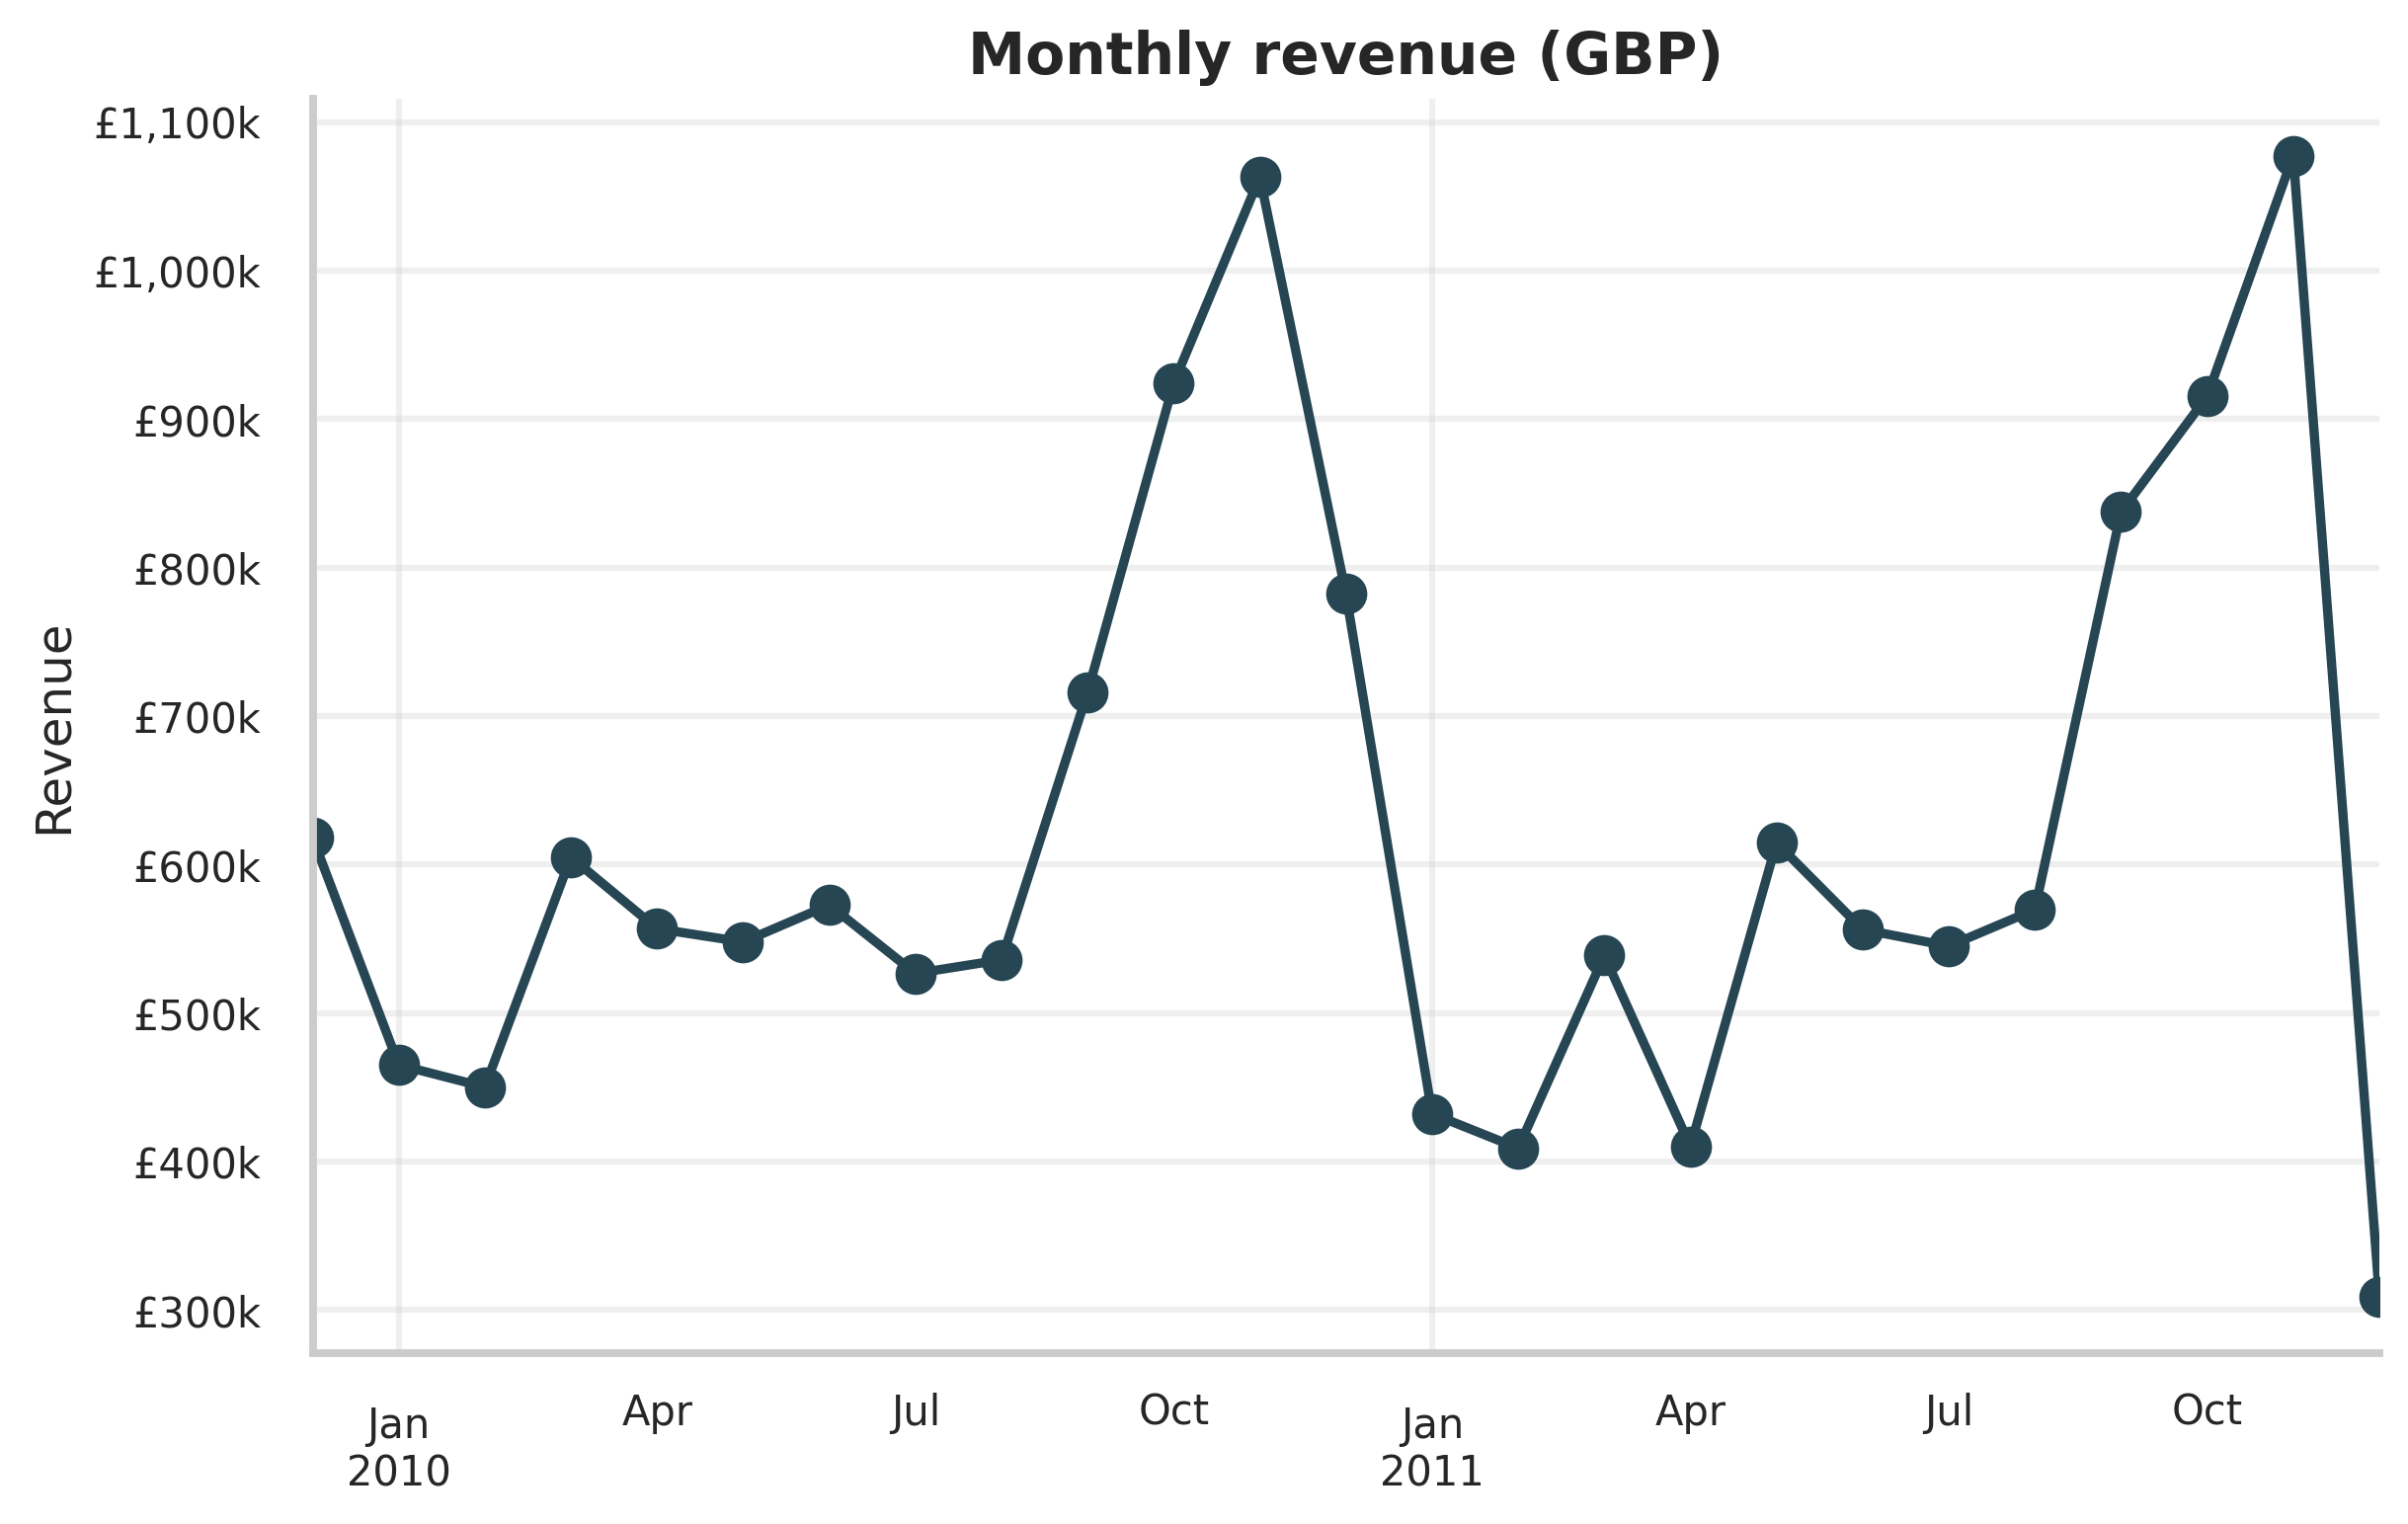
\includegraphics[width=\linewidth]{figures/01_monthly_revenue.png}
  \caption{Monthly revenue (GBP) from cleaned Online Retail II transactions.}
  \label{fig:eda}
\end{figure}

\subsection{Customer segmentation}
The joint elbow/silhouette sweep over $k=2..10$ (Figure~\ref{fig:sweep}) selects $k=2$ as optimal for K-means; AGNES is cut at the same $k$. DBSCAN, with $\varepsilon$ chosen from the 92nd percentile of the 4-NN distance plot, fragments the space into 13 small clusters plus 403 noise points and is dominated on every index (Table~\ref{tab:clusters}). The two K-means segments are easily interpretable: \textit{Dormant} (cluster~0, $n{=}3{,}189$, 54.3\%, mean Recency 317 d, Frequency 1.9, Monetary \pounds 496) and \textit{Active loyal} (cluster~1, $n{=}2{,}689$, 45.7\%, mean Recency 63 d, Frequency 11.6, Monetary \pounds 5{,}206). Across 10 random seeds the K-means silhouette is stable at {{clustering_silhouette}} (std {{clustering_silhouette_std}}). Figure~\ref{fig:clust} shows the K-means partition projected to two PCA components.

\begin{table}[t]
\caption{Internal validation of the three clustering algorithms (best per metric in bold).}
\label{tab:clusters}
\centering
\begin{tabular}{lrrrr}
\toprule
Algorithm & $k$ & Silhouette $\uparrow$ & Davies--Bouldin $\downarrow$ & Calinski--Harabasz $\uparrow$ \\
\midrule
K-means & 2  & \textbf{0.419}  & 0.886 & \textbf{5{,}840} \\
DBSCAN  & 13 & $-0.121$        & 1.632 & 742              \\
AGNES   & 2  & 0.388           & \textbf{0.789} & 4{,}304 \\
\bottomrule
\end{tabular}
\end{table}

\begin{figure}[t]
  \centering
  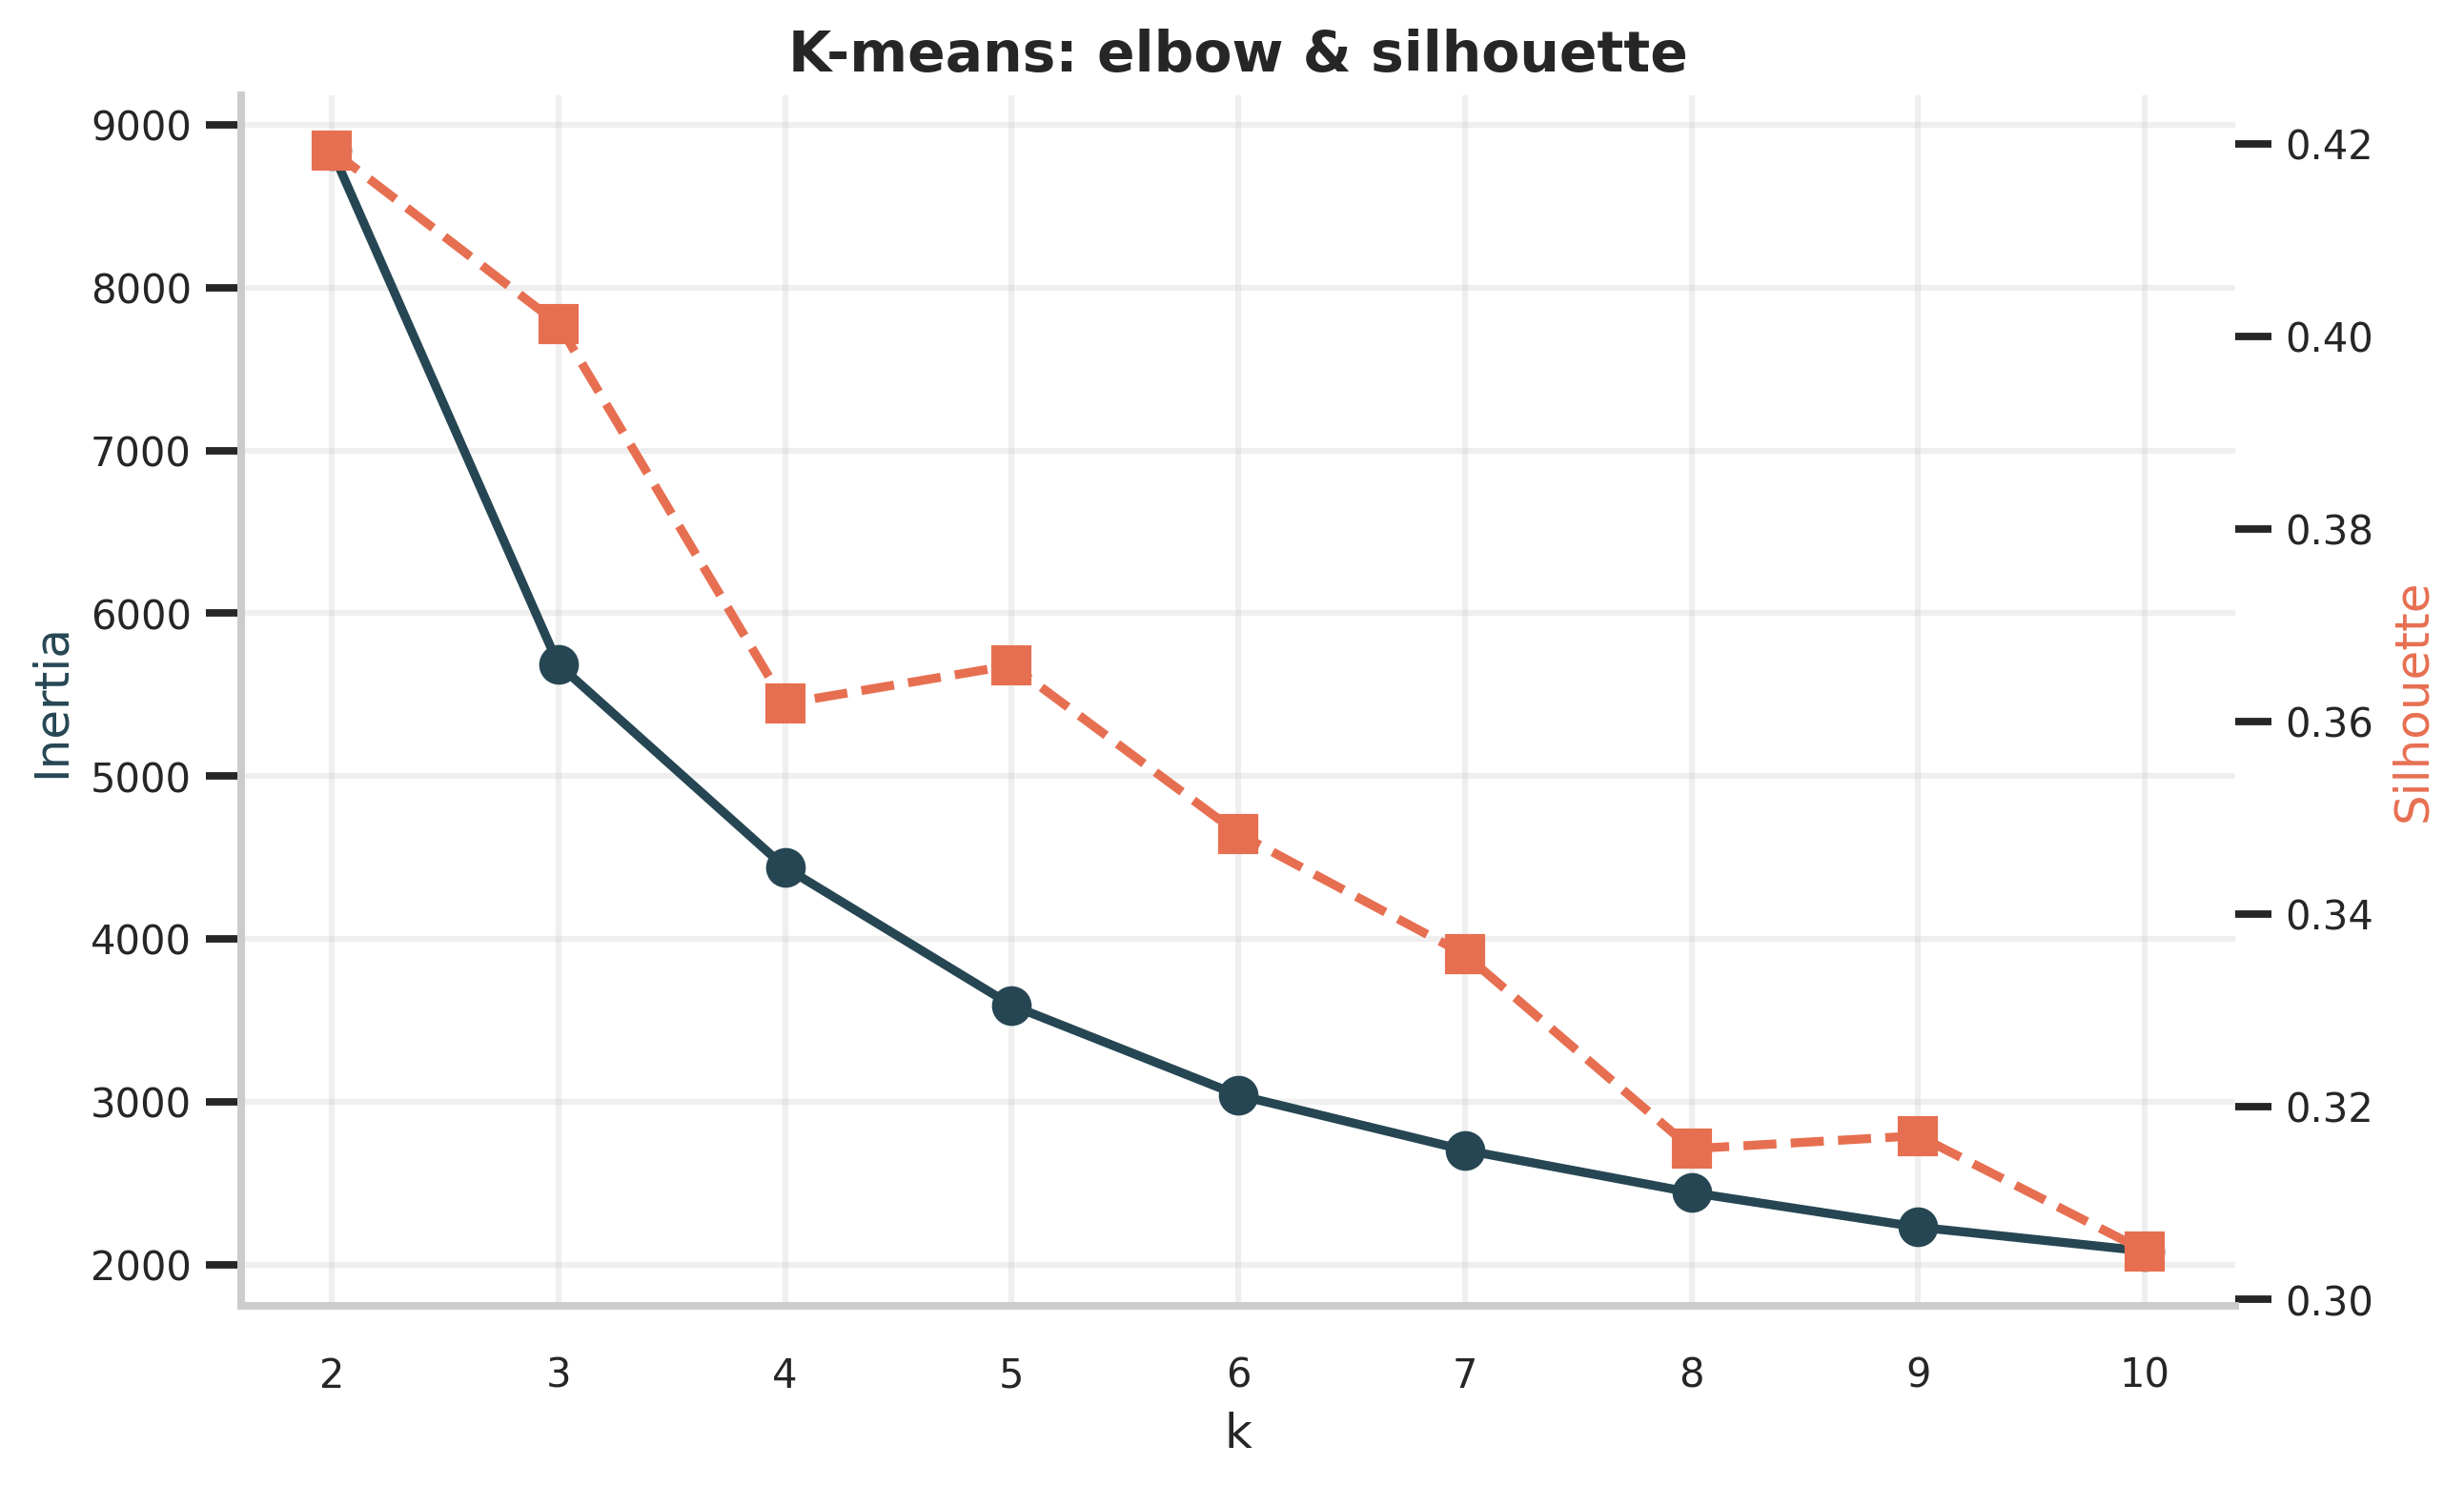
\includegraphics[width=\linewidth]{figures/02_kmeans_sweep.png}
  \caption{Model selection for K-means: elbow (inertia) and silhouette over $k=2..10$. Silhouette peaks at $k=2$.}
  \label{fig:sweep}
\end{figure}

\begin{figure}[t]
  \centering
  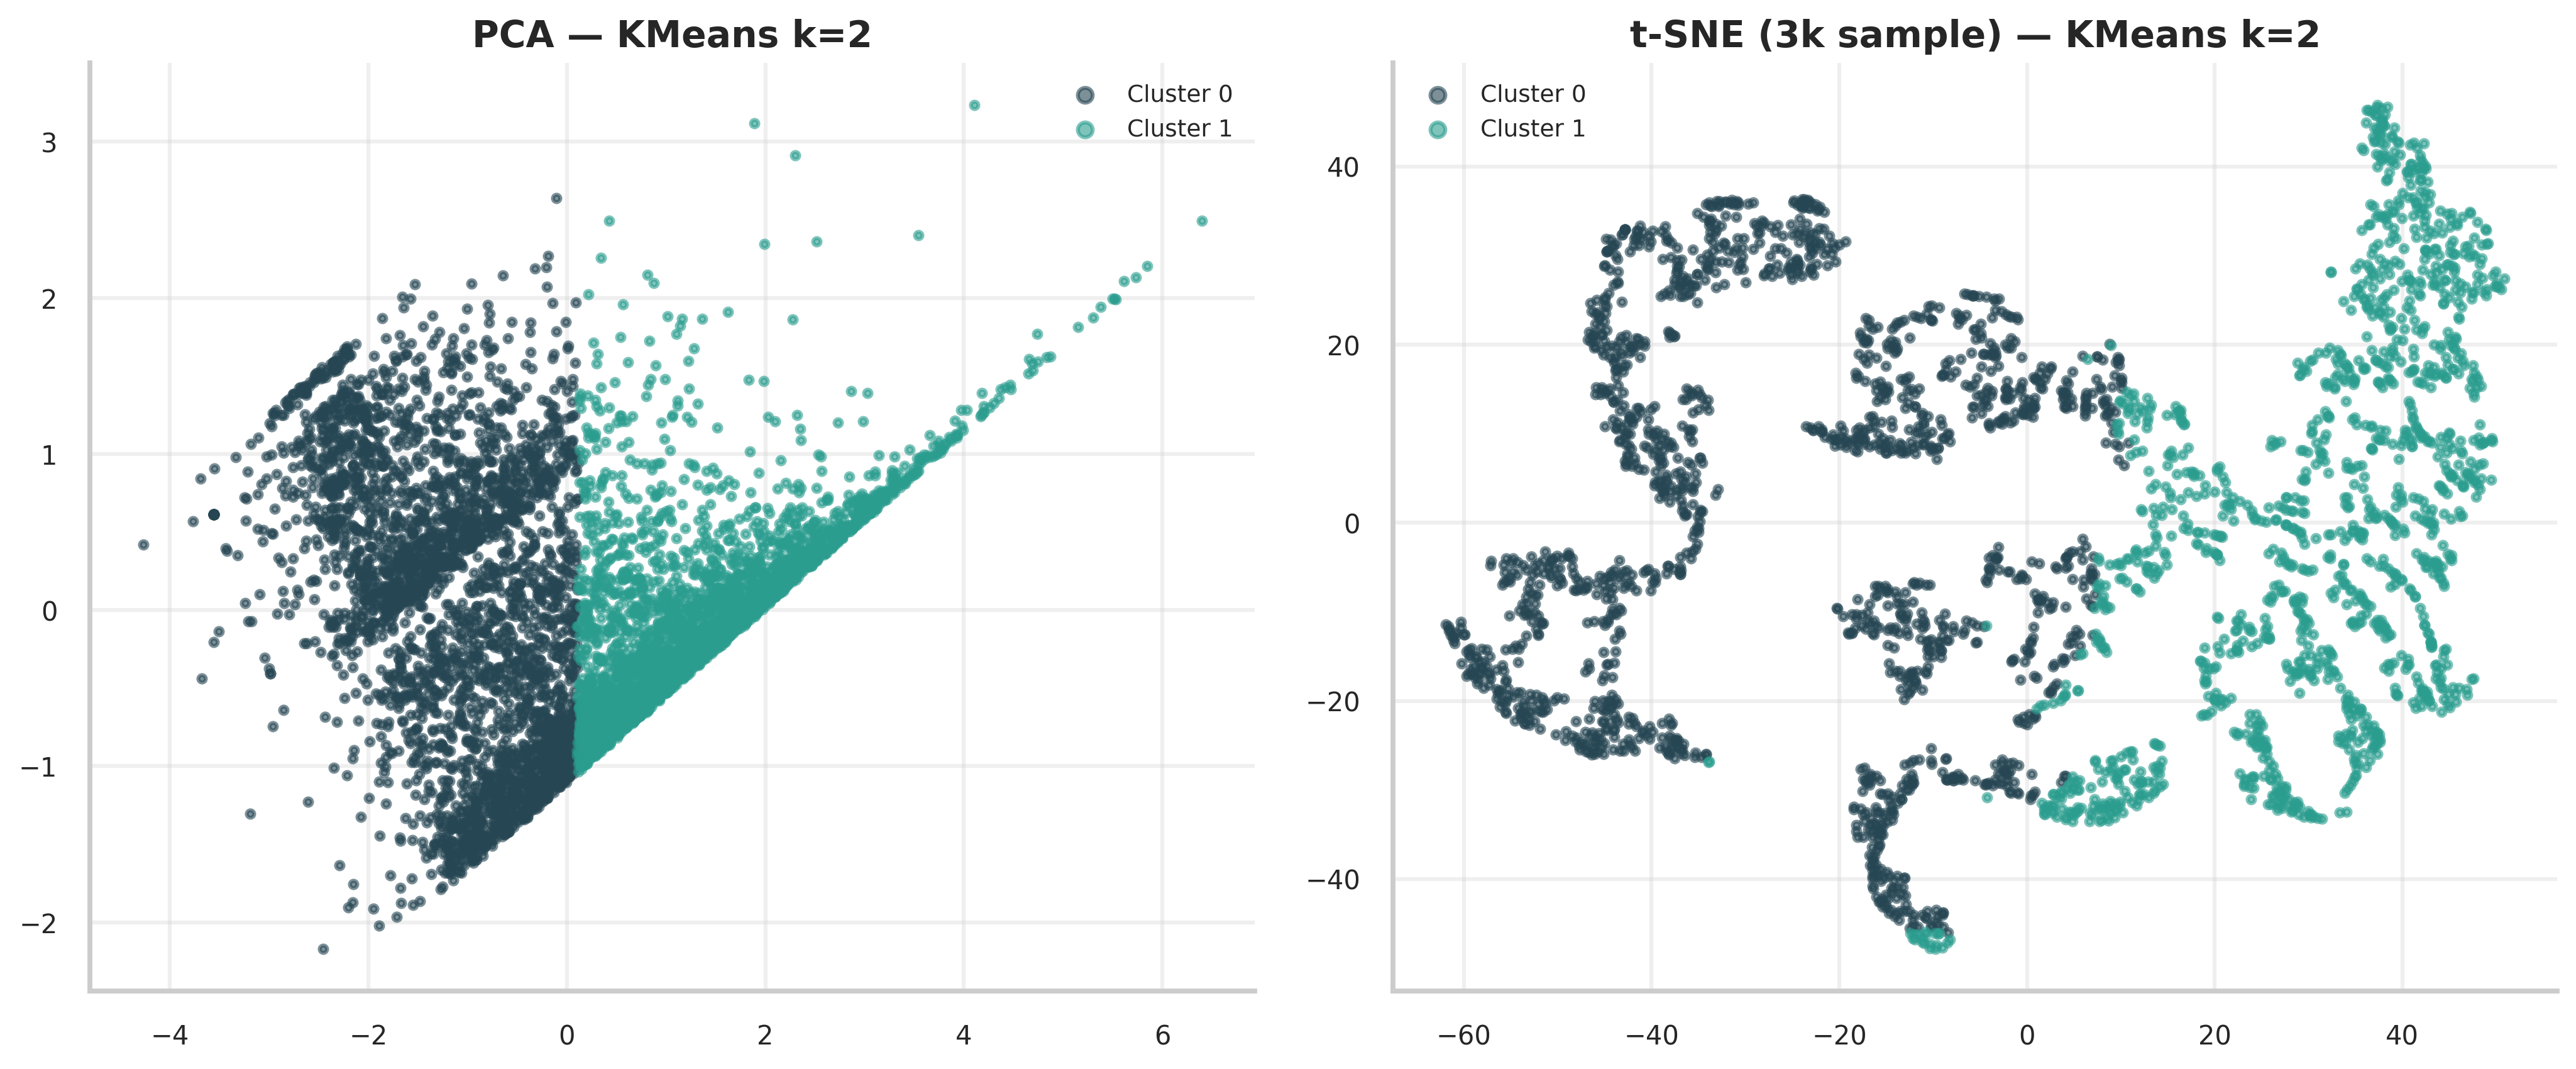
\includegraphics[width=\linewidth]{figures/02_pca_tsne.png}
  \caption{K-means segmentation visualised with PCA (left) and t-SNE (right, $n{=}3$k subsample). The two segments separate cleanly on the first PCA component.}
  \label{fig:clust}
\end{figure}

\subsection{Churn classification}
Among the {{n_customers_labelled}} customers active before the {{churn_cutoff}} cutoff, {{churn_rate}} are labelled \emph{churned} (no purchase in the following {{churn_window_days}} days). Table~\ref{tab:classification} reports held-out test scores; the ROC overlay (Figure~\ref{fig:roc}) makes the ordering visually unambiguous. {{classification_best_model}} leads with AUC {{classification_best_auc}} (5-fold CV {{classification_best_cv_auc}}) and the MLP reaches {{classification_mlp_auc}}; all models cluster within roughly 0.03 AUC. This realistic range is expected: every supervised feature is computed strictly before the cutoff and preprocessing (scaling and country one-hot encoding) is fit only on the training folds, eliminating the target leakage that otherwise inflates these scores to near 0.99. We retain Recency---always available at scoring time---and isolate its contribution by ablation in Section~V.

\begin{table}[t]
\caption{Held-out test performance of churn classifiers (best in bold).}
\label{tab:classification}
\centering
\begin{tabular}{lrrrr}
\toprule
Model & AUC & F1 & Precision & Recall \\
\midrule
{{classification_table_body}}
\bottomrule
\end{tabular}
\end{table}

\begin{figure}[t]
  \centering
  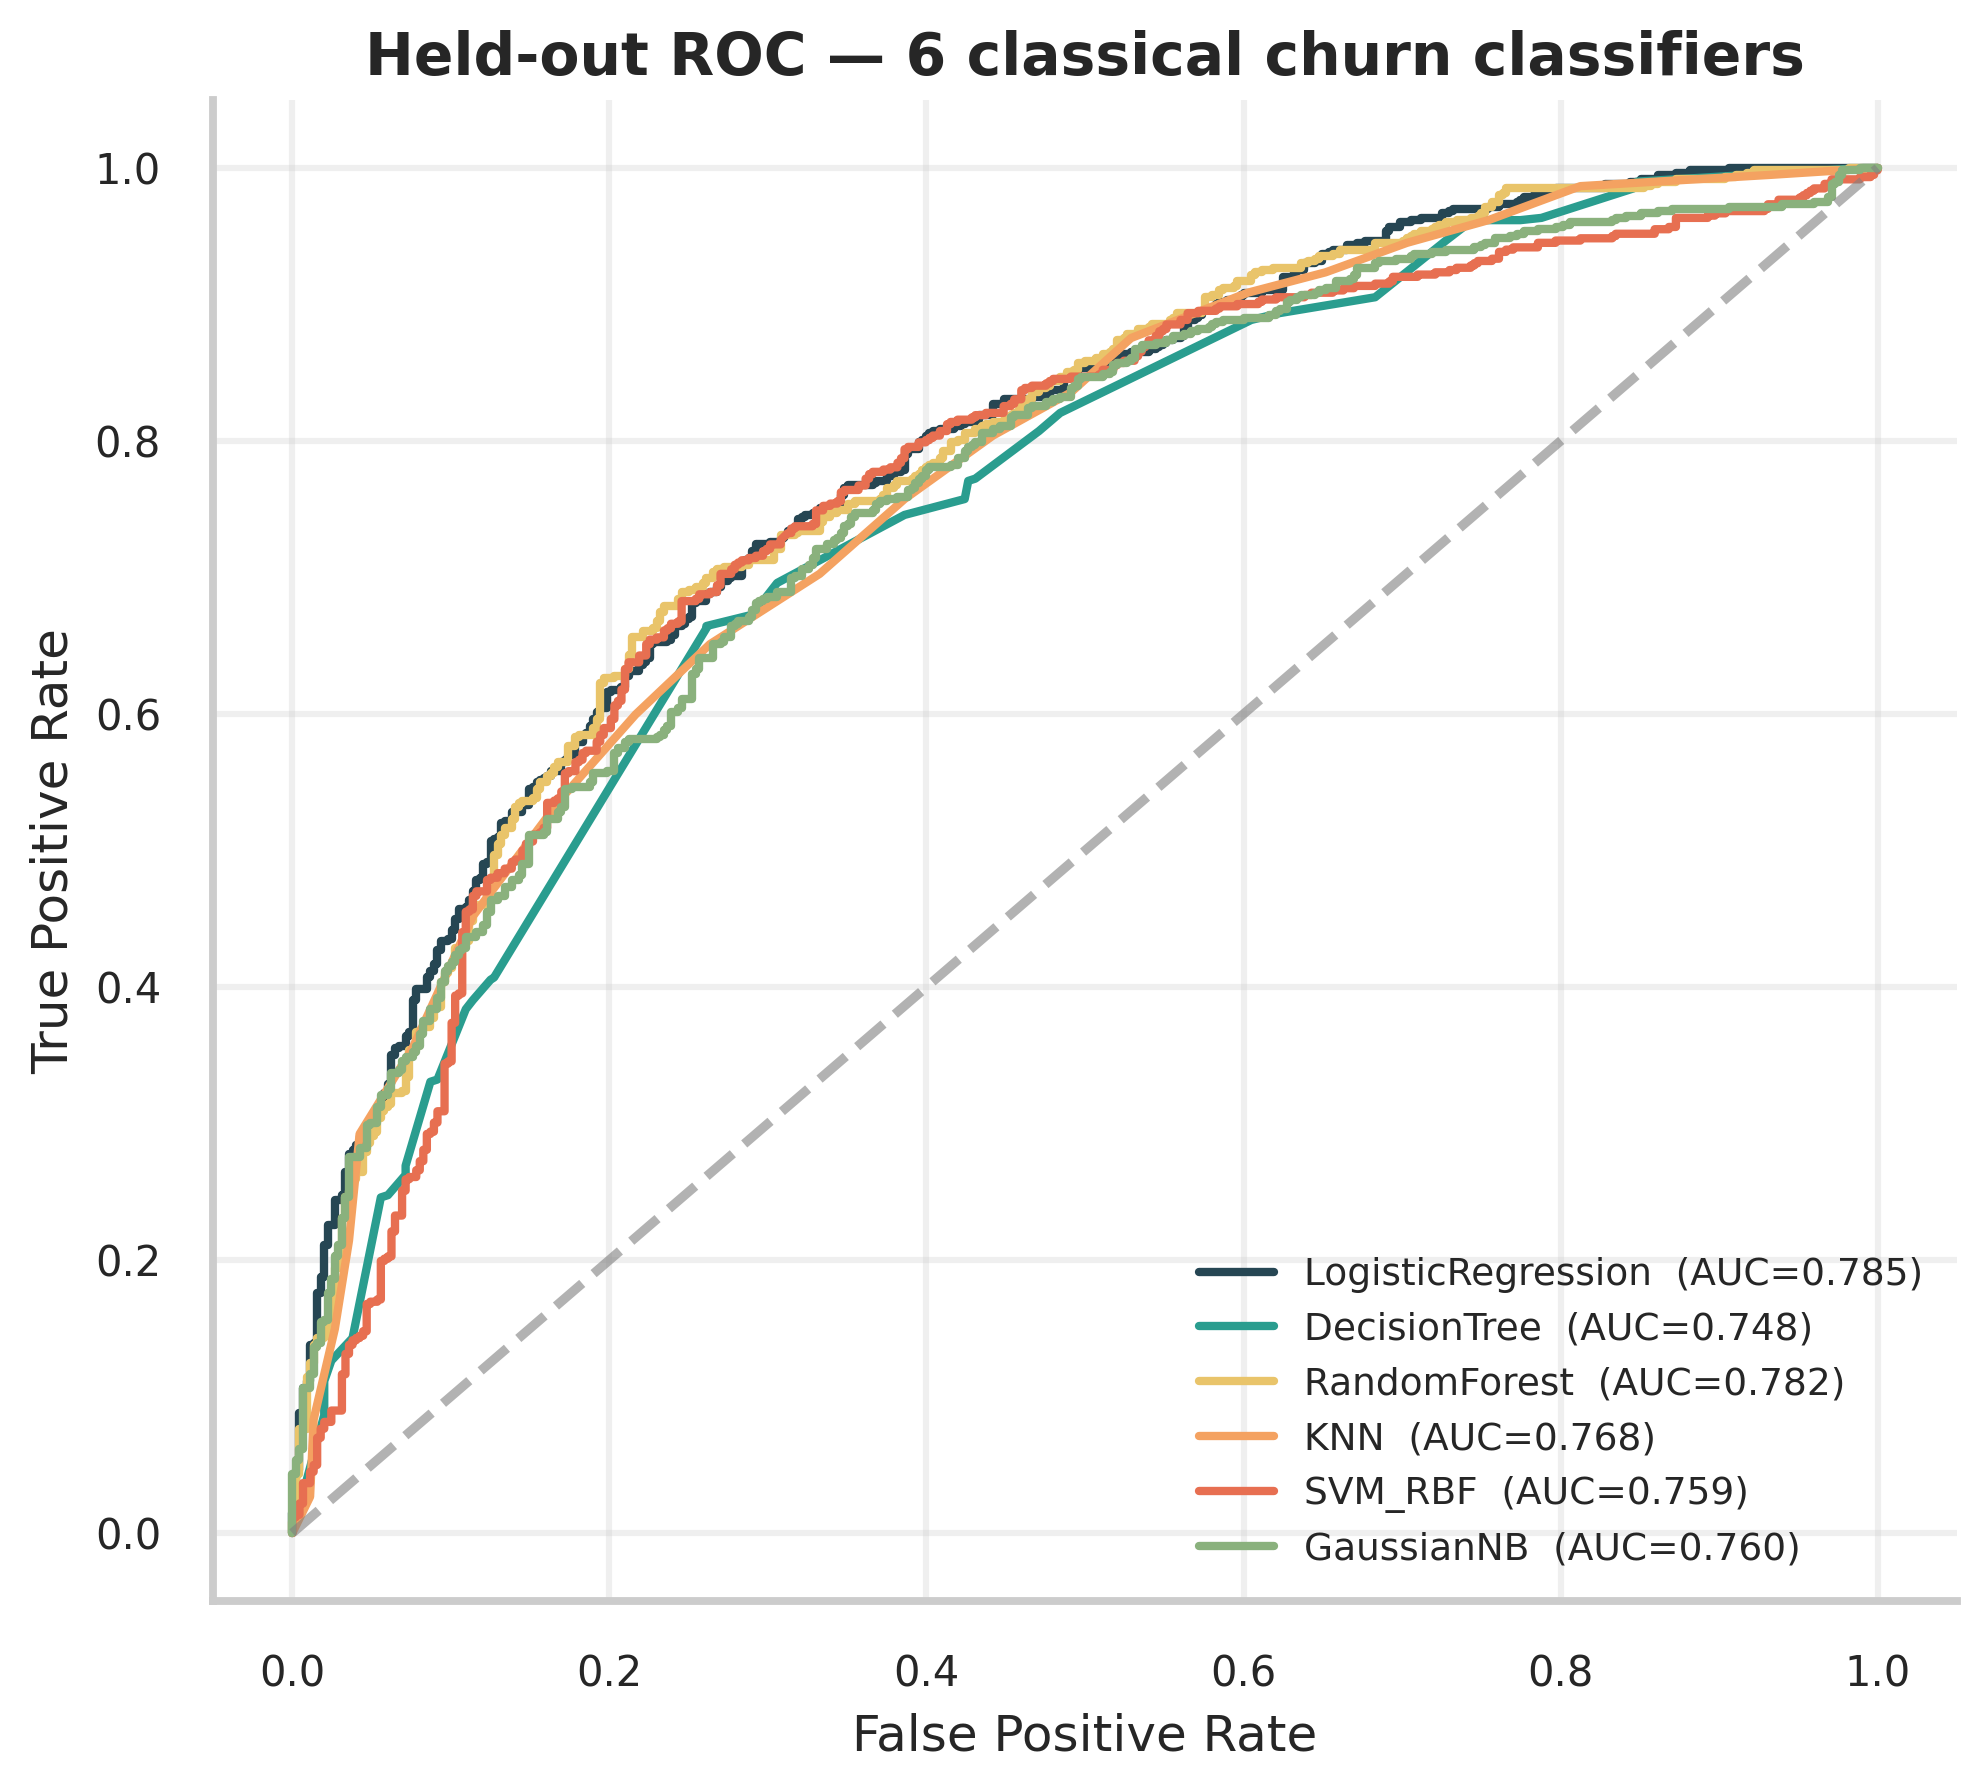
\includegraphics[width=\linewidth]{figures/03_roc_classical.png}
  \caption{Held-out ROC curves for the six classical churn classifiers.}
  \label{fig:roc}
\end{figure}

\textbf{Honest evaluation.} To confirm the classifier learns genuine churn signal rather than merely echoing Recency, we benchmark it against honest baselines (Table~\ref{tab:baselines}) and ablate feature groups (Table~\ref{tab:ablation}). The full model (AUC {{classification_best_auc}}) clearly beats a majority-class predictor (0.500) and a recency-only model (0.751), and dropping Recency lowers the AUC only to 0.755---so Recency is dominant but \emph{not} sufficient, and the behavioural features add real signal. The predicted probabilities are also well calibrated (Brier {{calibration_brier}}): the reliability curve in Figure~\ref{fig:calib} hugs the diagonal, which matters because the downstream decision layer thresholds directly on these probabilities.

\begin{table}[t]
\caption{Honest baselines for churn (held-out AUC). The full model is benchmarked against trivial and reduced-feature predictors.}
\label{tab:baselines}
\centering
\begin{tabular}{lrr}
\toprule
Baseline & \# feat. & AUC \\
\midrule
Majority class                     & ---  & 0.500 \\
Recency only (LogReg)              & 1    & 0.751 \\
All features, no Recency (LogReg)  & 6    & 0.755 \\
\midrule
\textbf{Best model (LogReg, all feat.)} & 7 & \textbf{0.785} \\
\bottomrule
\end{tabular}
\end{table}

\begin{table}[t]
\caption{Feature-group ablation (5-fold CV and held-out test AUC). RFM is the backbone; adding behavioural features helps, Country does not, and removing Recency hurts most.}
\label{tab:ablation}
\centering
\begin{tabular}{lrrr}
\toprule
Feature group & \# feat. & CV AUC & Test AUC \\
\midrule
RFM only                       & 3 & 0.797 & 0.784 \\
Behavioural only               & 3 & 0.719 & 0.720 \\
RFM + Behavioural              & 6 & \textbf{0.798} & \textbf{0.787} \\
RFM + Behavioural + Country    & 7 & 0.798 & 0.784 \\
Without Recency                & 6 & 0.762 & 0.755 \\
\bottomrule
\end{tabular}
\end{table}

\begin{figure}[t]
  \centering
  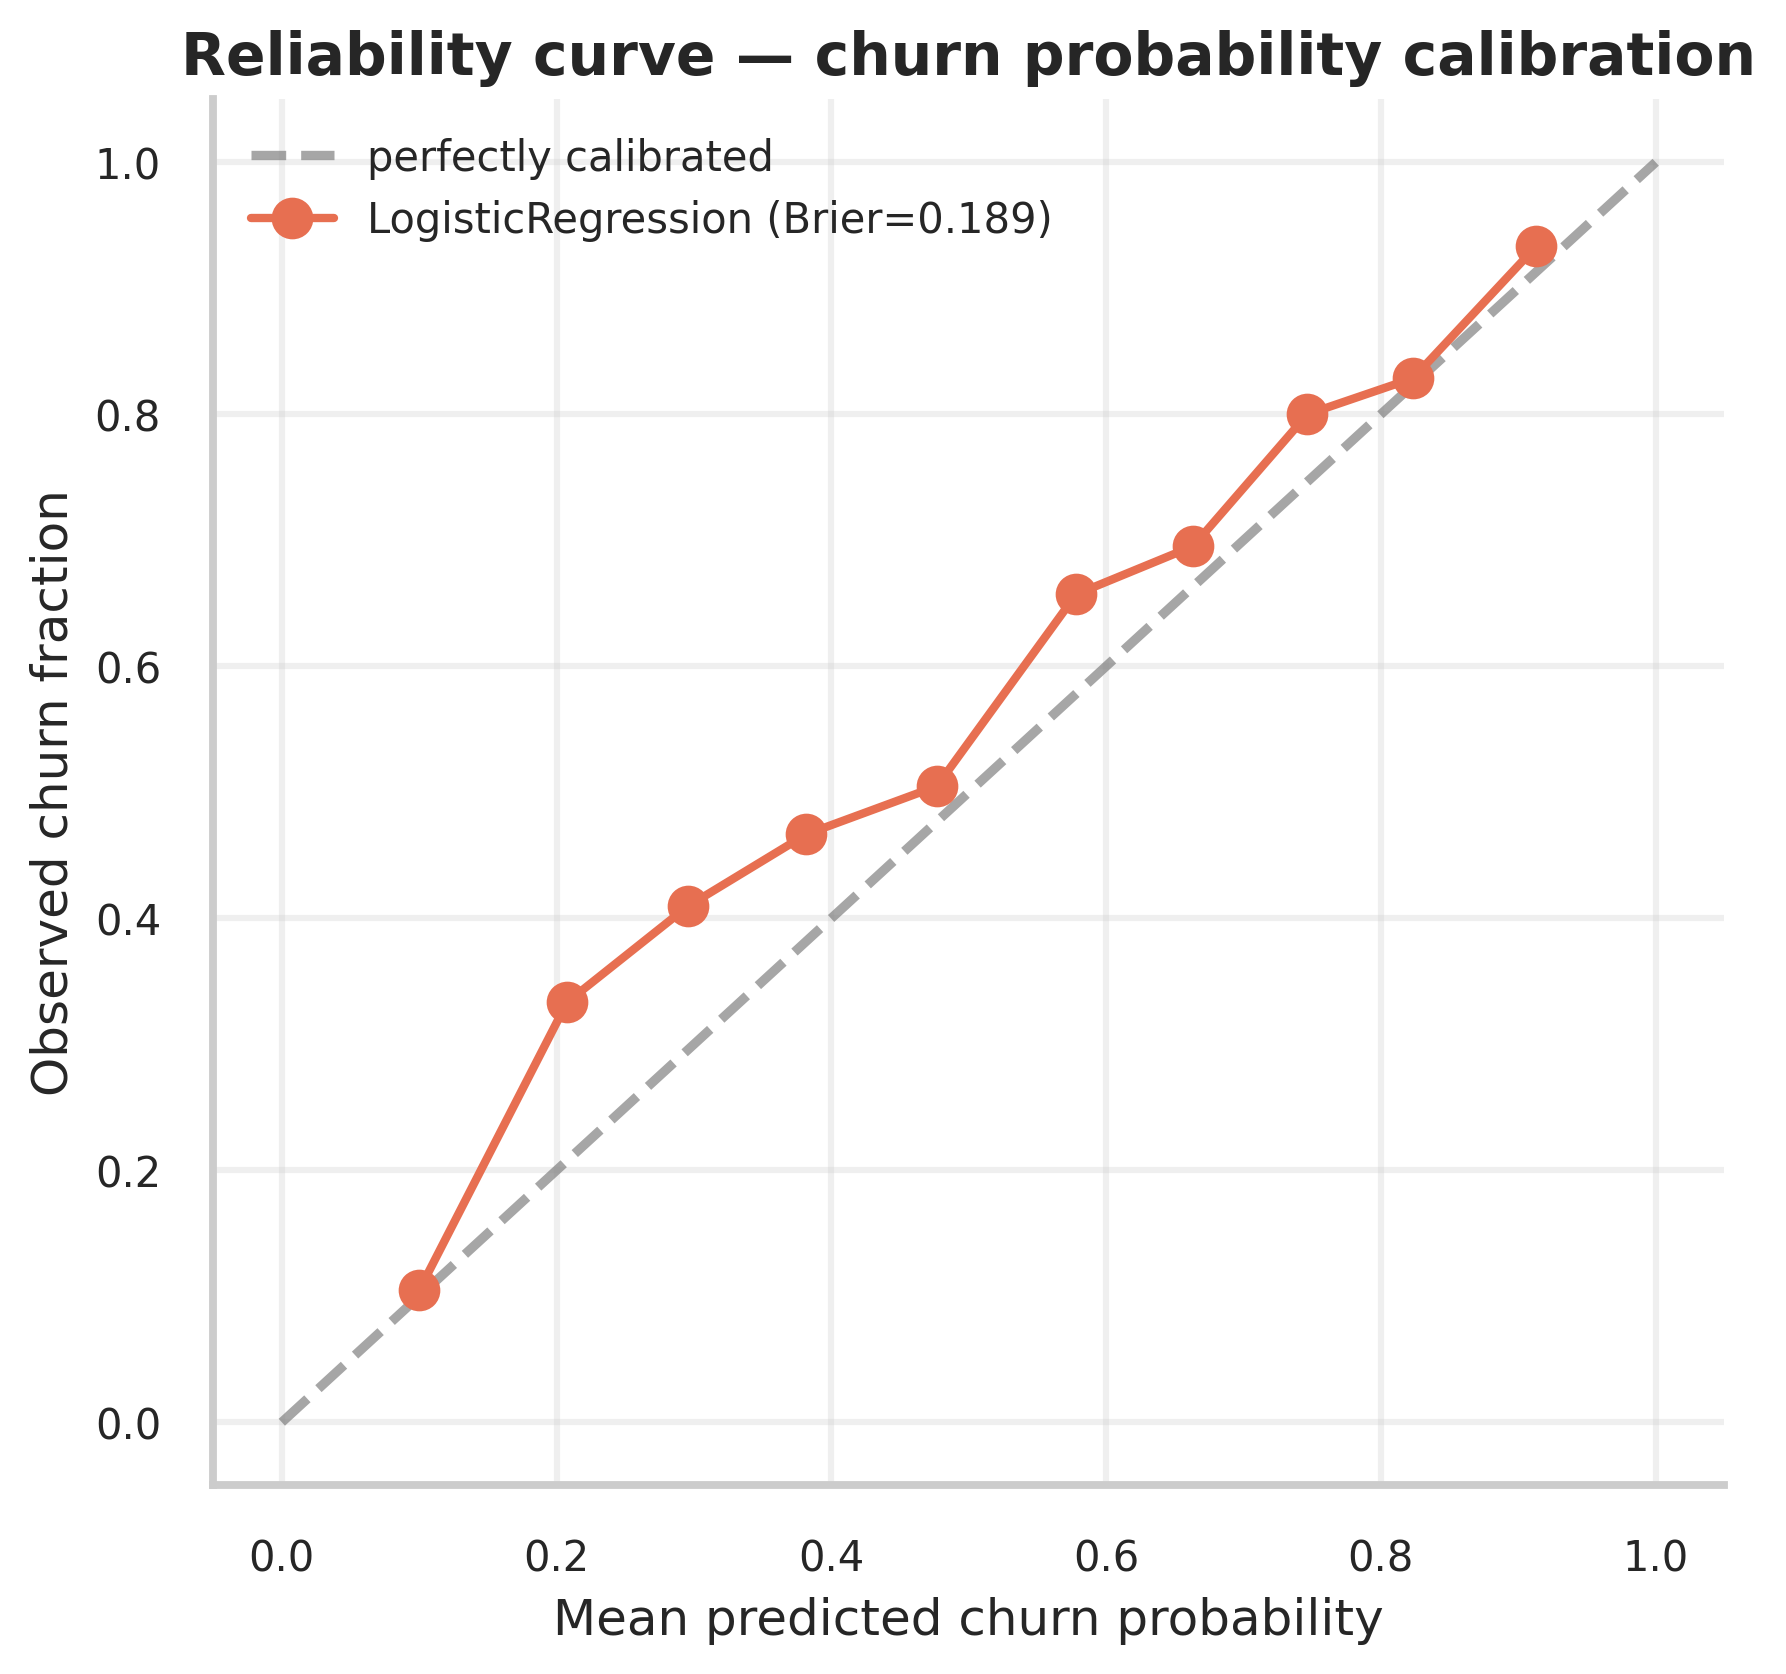
\includegraphics[width=\linewidth]{figures/03_calibration.png}
  \caption{Reliability curve for the {{classification_best_model}} churn model (10 bins). Predicted probabilities track observed churn frequency closely (Brier {{calibration_brier}}).}
  \label{fig:calib}
\end{figure}

\subsection{Association rules}
Restricting to the stock codes appearing in at least 0.5\% of invoices, Apriori and FP-Growth mine an identical set of 242 frequent itemsets at $\min\_support=0.02$. After applying $\min\_confidence=0.5$ and $\min\_lift=1.5$, {{association_n_rules}} rules remain. Apriori takes 6.08~s on this candidate space; FP-Growth completes the same workload in 4.15~s, a 1.5$\times$ speedup (Figure~\ref{fig:assocrt}). The top rules in Table~\ref{tab:rules} reveal that the strongest co-purchase signals correspond to collectible \emph{sets} (Regency teacup pair, lift {{top_rule_lift}}) and color-coordinated variants of the same product (lunchbags, jumbo bags, heart t-light holders), patterns we exploit in the cross-task synthesis. Figure~\ref{fig:rules} shows the top-20 rules as a co-occurrence network.

\begin{table}[t]
\caption{Top five association rules by lift (FP-Growth, after redundancy pruning).}
\label{tab:rules}
\centering
\footnotesize
\begin{tabular}{p{2.5cm}p{2.5cm}rr}
\toprule
Antecedent & Consequent & Conf. & Lift \\
\midrule
Roses Regency Teacup            & Green Regency Teacup            & 0.70 & 26.8 \\
Green Regency Teacup            & Roses Regency Teacup            & 0.80 & 26.8 \\
Sweetheart Ceramic Trinket Box  & Strawberry Ceramic Trinket Box  & 0.73 & 13.9 \\
Wooden Picture Frame White      & Wooden Frame Antique White      & 0.60 & 12.1 \\
Wooden Frame Antique White      & Wooden Picture Frame White      & 0.56 & 12.1 \\
\bottomrule
\end{tabular}
\end{table}

\begin{figure}[t]
  \centering
  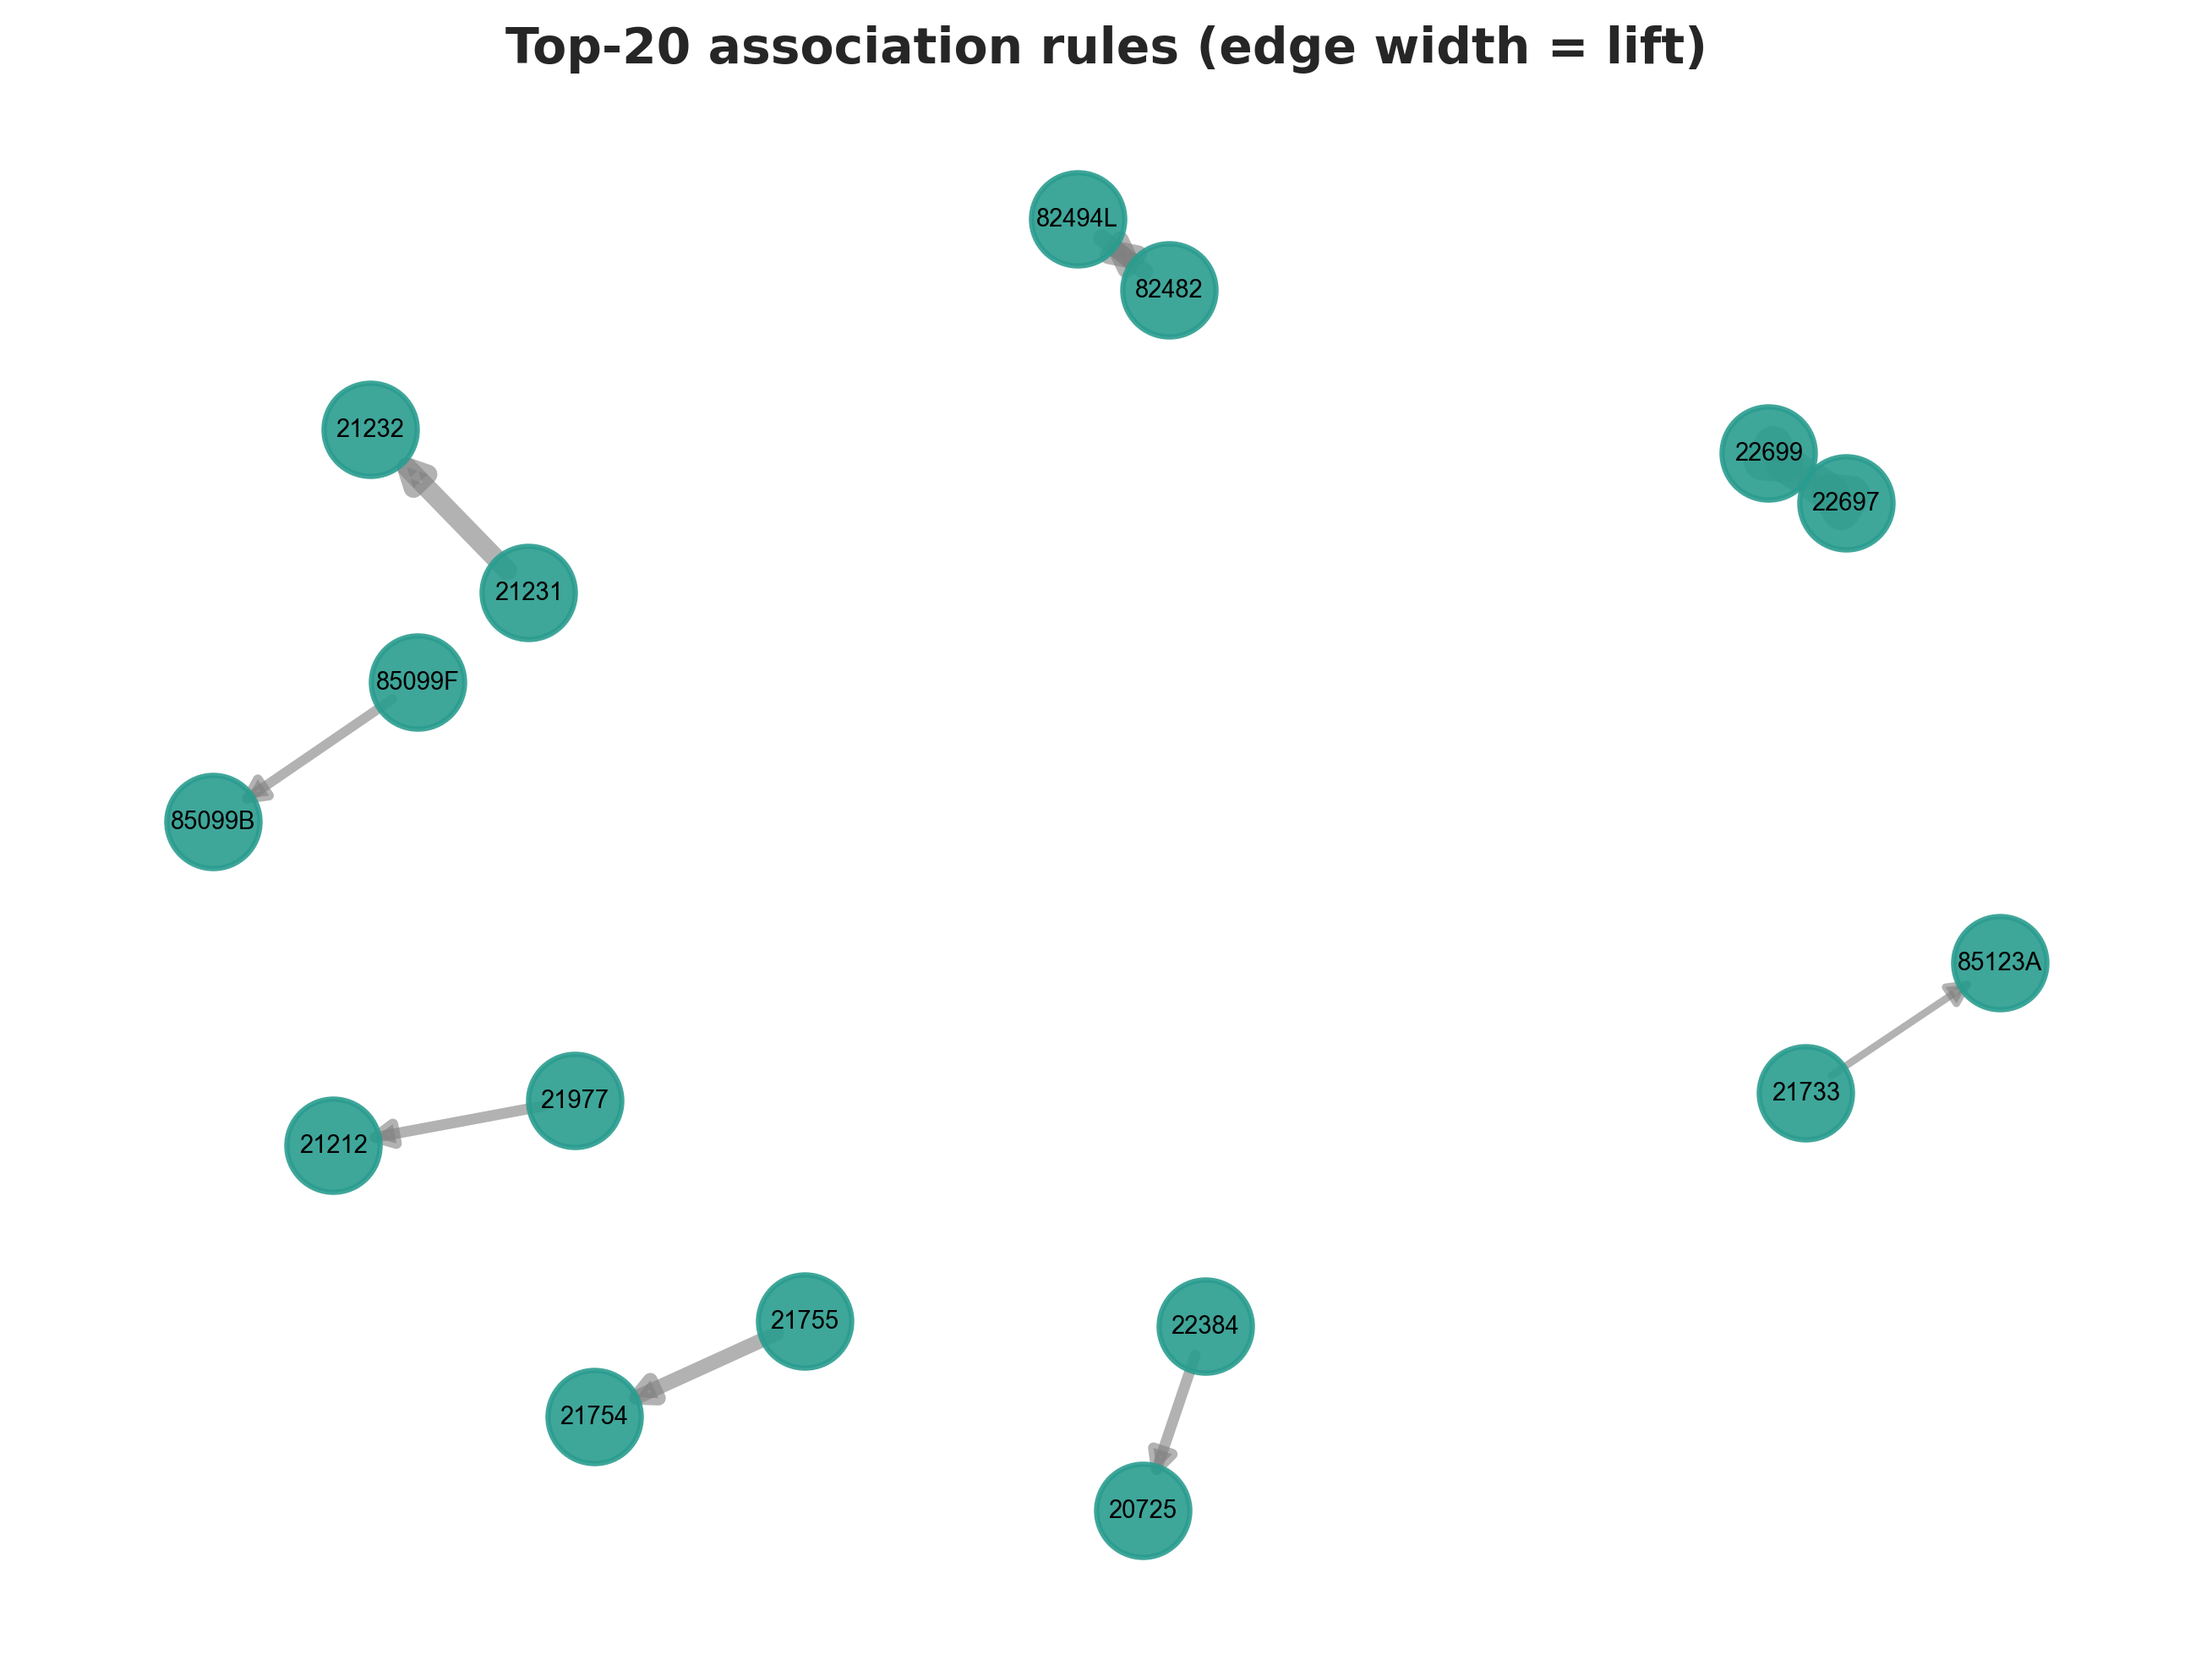
\includegraphics[width=\linewidth]{figures/04_rule_network.png}
  \caption{Top-20 association rules as a directed network; edge width $\propto$ lift.}
  \label{fig:rules}
\end{figure}

\begin{figure}[t]
  \centering
  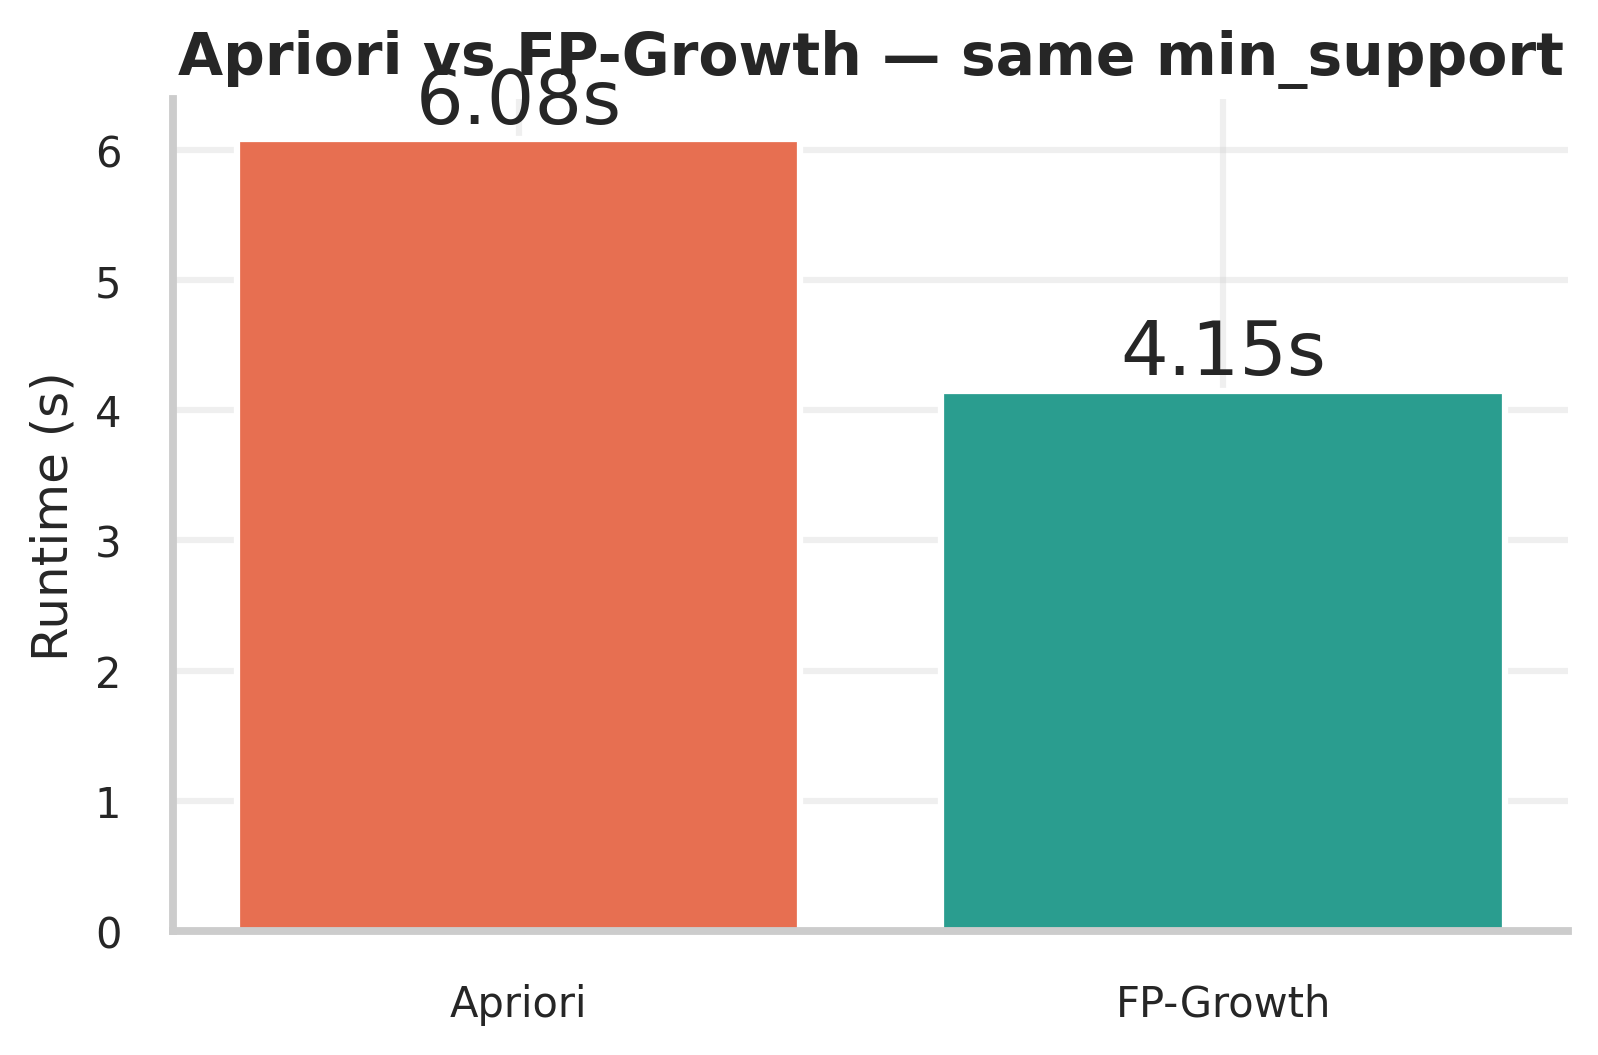
\includegraphics[width=\linewidth]{figures/04_apriori_vs_fpgrowth.png}
  \caption{Apriori vs FP-Growth on identical parameters: same 242 itemsets and 17 rules, but FP-Growth is $\approx$1.5$\times$ faster.}
  \label{fig:assocrt}
\end{figure}

\subsection{Explainability and anomaly detection}
The SHAP analysis (Figure~\ref{fig:shap}) confirms that Recency is by far the dominant churn driver, followed by Frequency and the behavioural variables; geographic one-hots contribute marginally. TreeExplainer (Random Forest) and KernelExplainer (MLP) agree on this ordering. The autoencoder converges within 80 epochs and yields a heavy right tail of reconstruction errors; the 95th-percentile threshold flags 263 anomalous customers (5\% of labelled customers, Figure~\ref{fig:ae}). Inspection shows these customers combine extremely high Frequency with atypical basket sizes --- candidates for either VIP outreach or fraud screening, depending on operational context.

\begin{figure}[t]
  \centering
  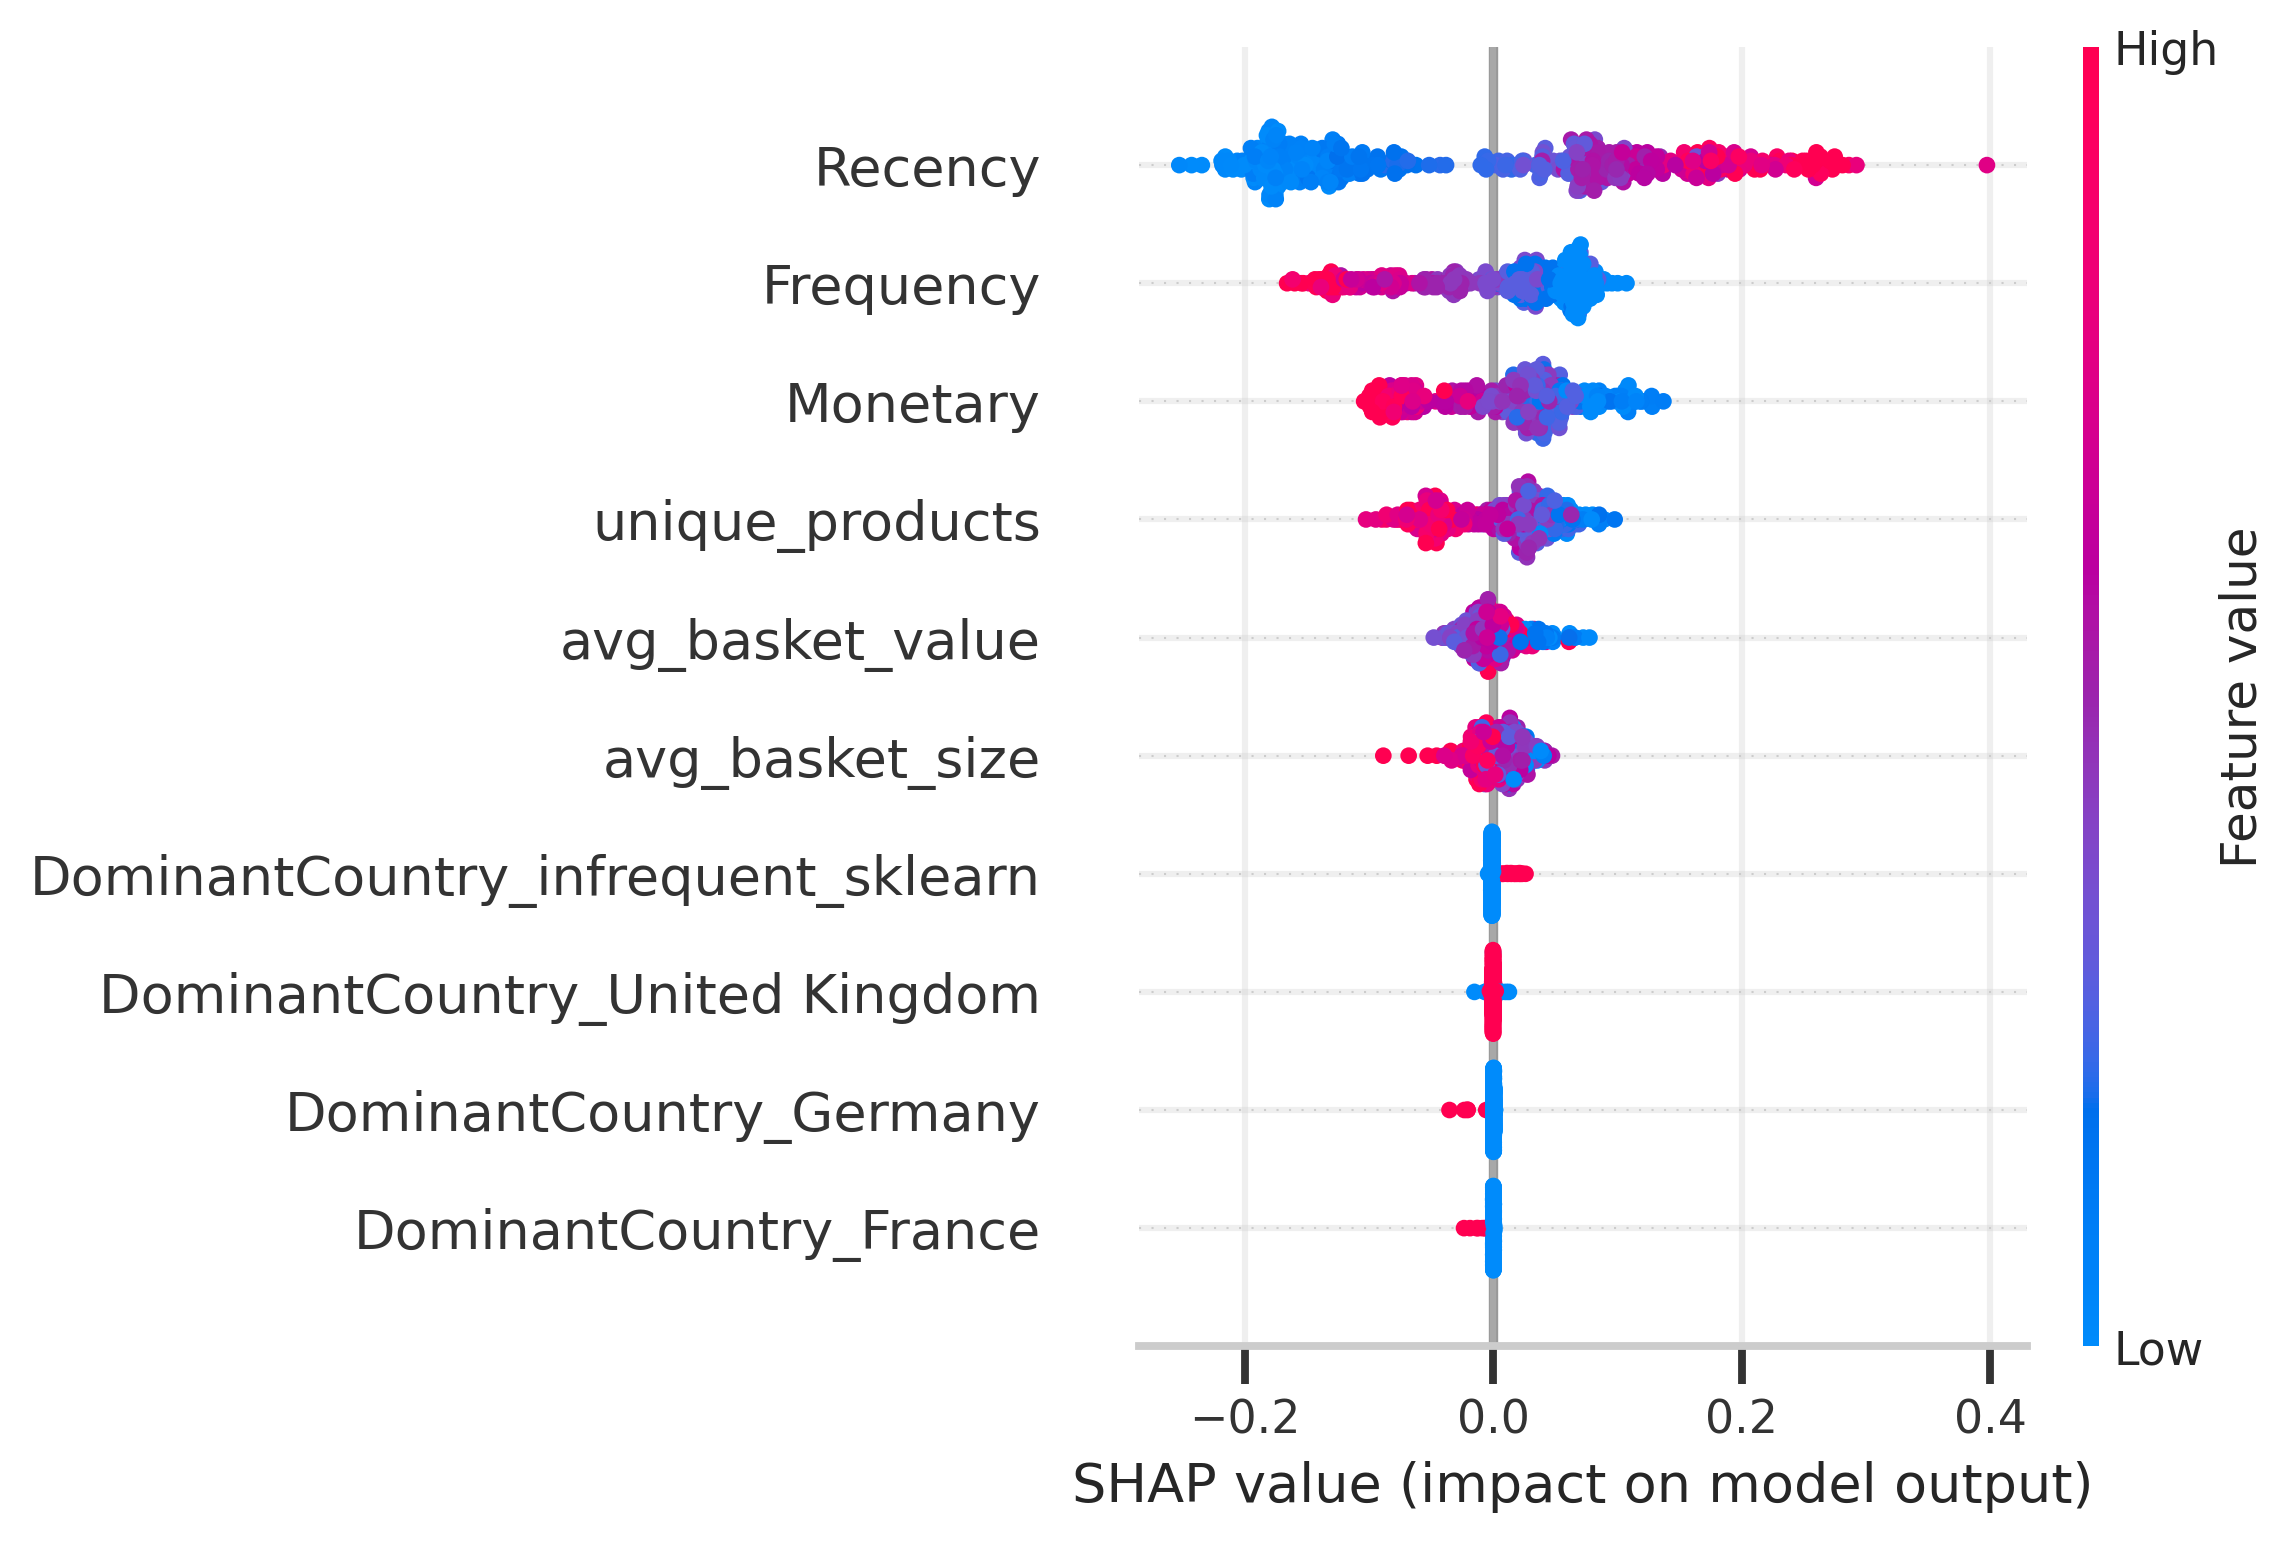
\includegraphics[width=\linewidth]{figures/05_shap_beeswarm.png}
  \caption{SHAP beeswarm for the RandomForest churn classifier (400-sample explanation set). Recency dominates; higher Recency (red) drives the prediction toward churn.}
  \label{fig:shap}
\end{figure}

\begin{figure}[t]
  \centering
  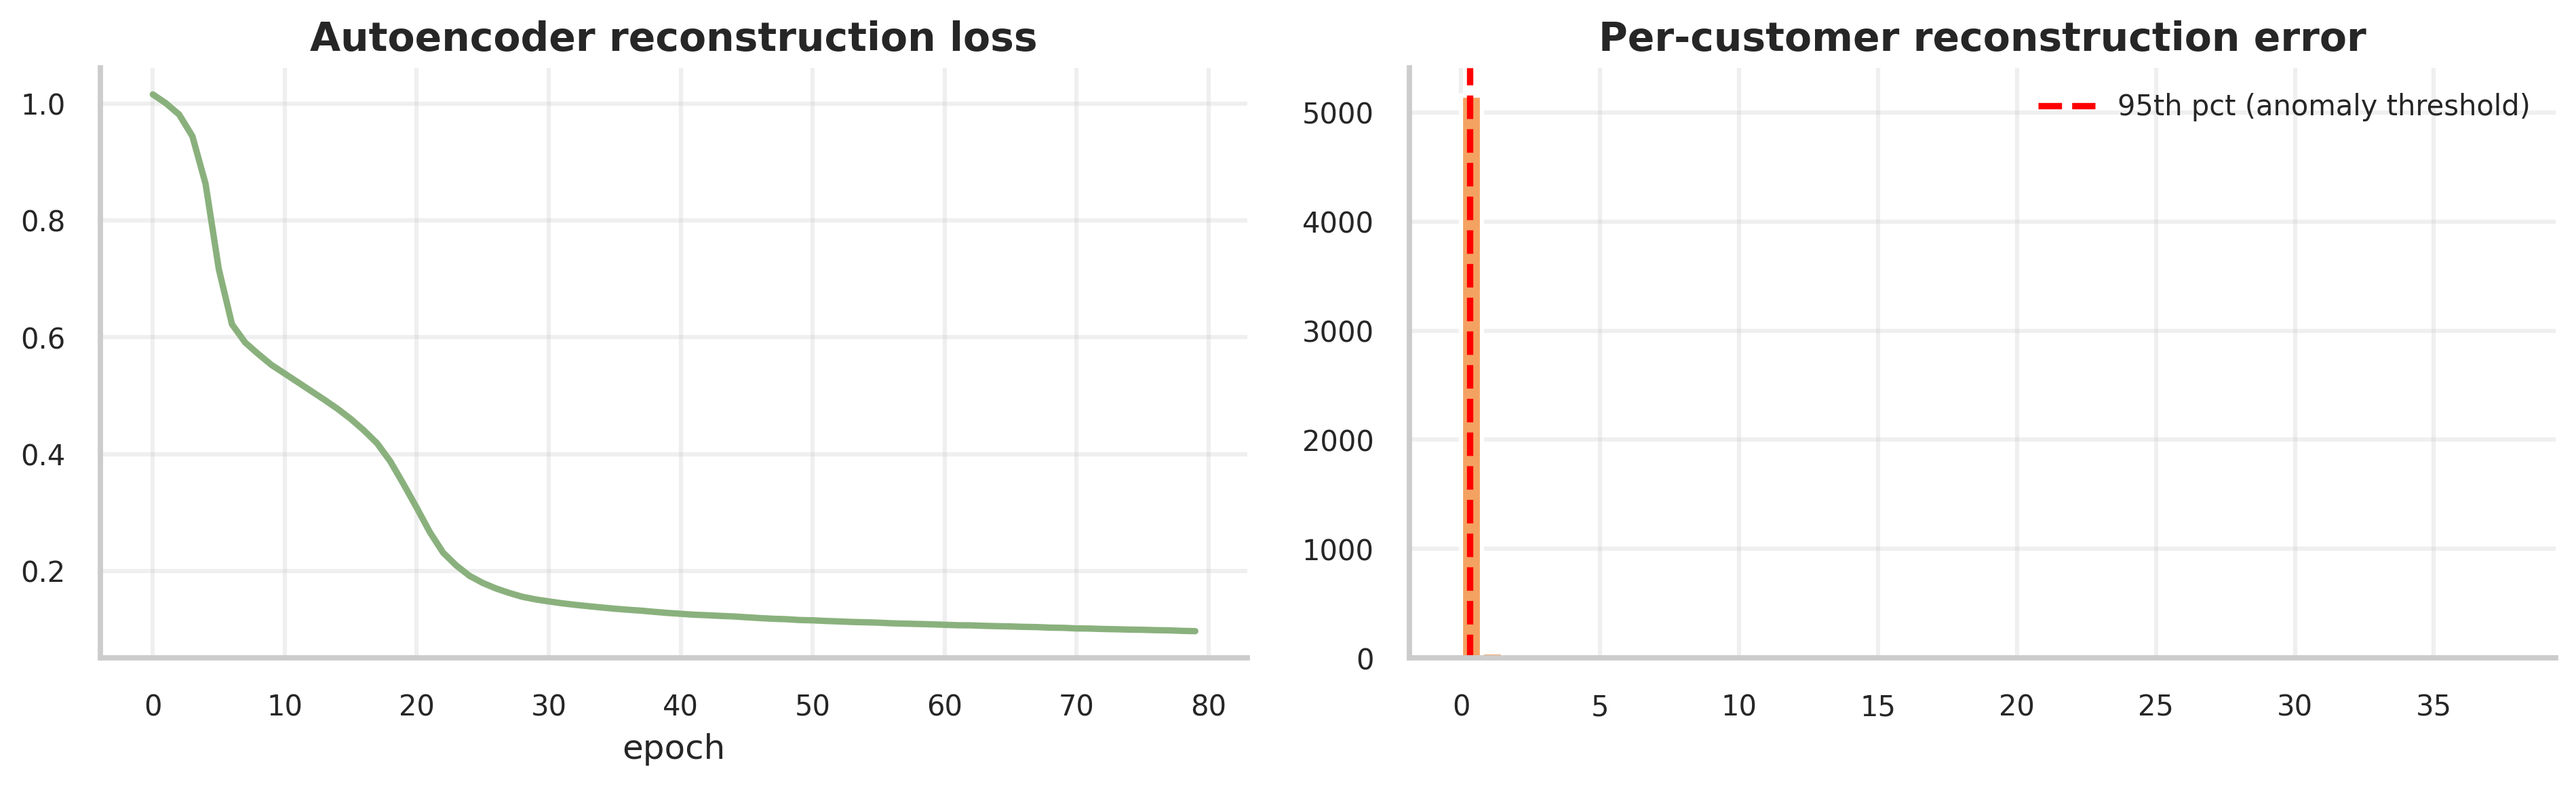
\includegraphics[width=\linewidth]{figures/05_autoencoder.png}
  \caption{Autoencoder reconstruction-error distribution. The heavy right tail beyond the 95th-percentile threshold (dashed) marks the 263 flagged anomalous customers.}
  \label{fig:ae}
\end{figure}

\subsection{Cross-task synthesis}
The cross-task analysis (Table~\ref{tab:synth} and Figure~\ref{fig:synth}) is the central contribution of this work: K-means segmentation, the churn label, and per-segment association mining are joined on \texttt{CustomerID}. The \textit{Dormant} segment carries a 90\% churn rate against 23\% for the \textit{Active loyal} segment, a {{churn_gap_points}}-percentage-point gap. Cluster-restricted FP-Growth recovers no rules for the dormant segment at the chosen thresholds (sparse baskets) but surfaces strong colour-coordinated co-purchase patterns within the loyal segment (the segment $\times$ top-product heatmap, Figure~\ref{fig:heatmap}) --- e.g., pink lunchbag $\to$ red lunchbag (lift 7.4), pink jumbo bag $\to$ red jumbo bag (lift 6.4), red heart t-light $\to$ white heart t-light (lift 5.3). The actionable recommendation: target the loyal segment's 23\% churners with color-pair bundles promoting the variants they have not yet purchased, and reserve broader win-back campaigns for the dormant majority. A downstream decision layer converts these signals into a per-customer action table covering all {{decision_table_customers}} scored customers ({{decision_retention_targets}} retention targets, {{decision_cross_sell_targets}} cross-sell, {{decision_manual_review_targets}} flagged for manual review), giving the business a single reproducible artifact for who to retain, grow, or review.

\begin{table}[t]
\caption{Churn rate and value per K-means segment.}
\label{tab:synth}
\centering
\begin{tabular}{lrrrr}
\toprule
Segment & $n$ & Churn \% & Avg.\ Recency & Avg.\ Monetary (\pounds) \\
\midrule
Dormant       & 2{,}697 & 90.0 & 367.9 &    519.5 \\
Active loyal  & 2{,}552 & 23.0 &  65.3 & 5{,}401.2 \\
\midrule
Overall       & {{n_customers_labelled}} & 57.4 & ---   & ---      \\
\bottomrule
\end{tabular}
\end{table}

\begin{figure}[t]
  \centering
  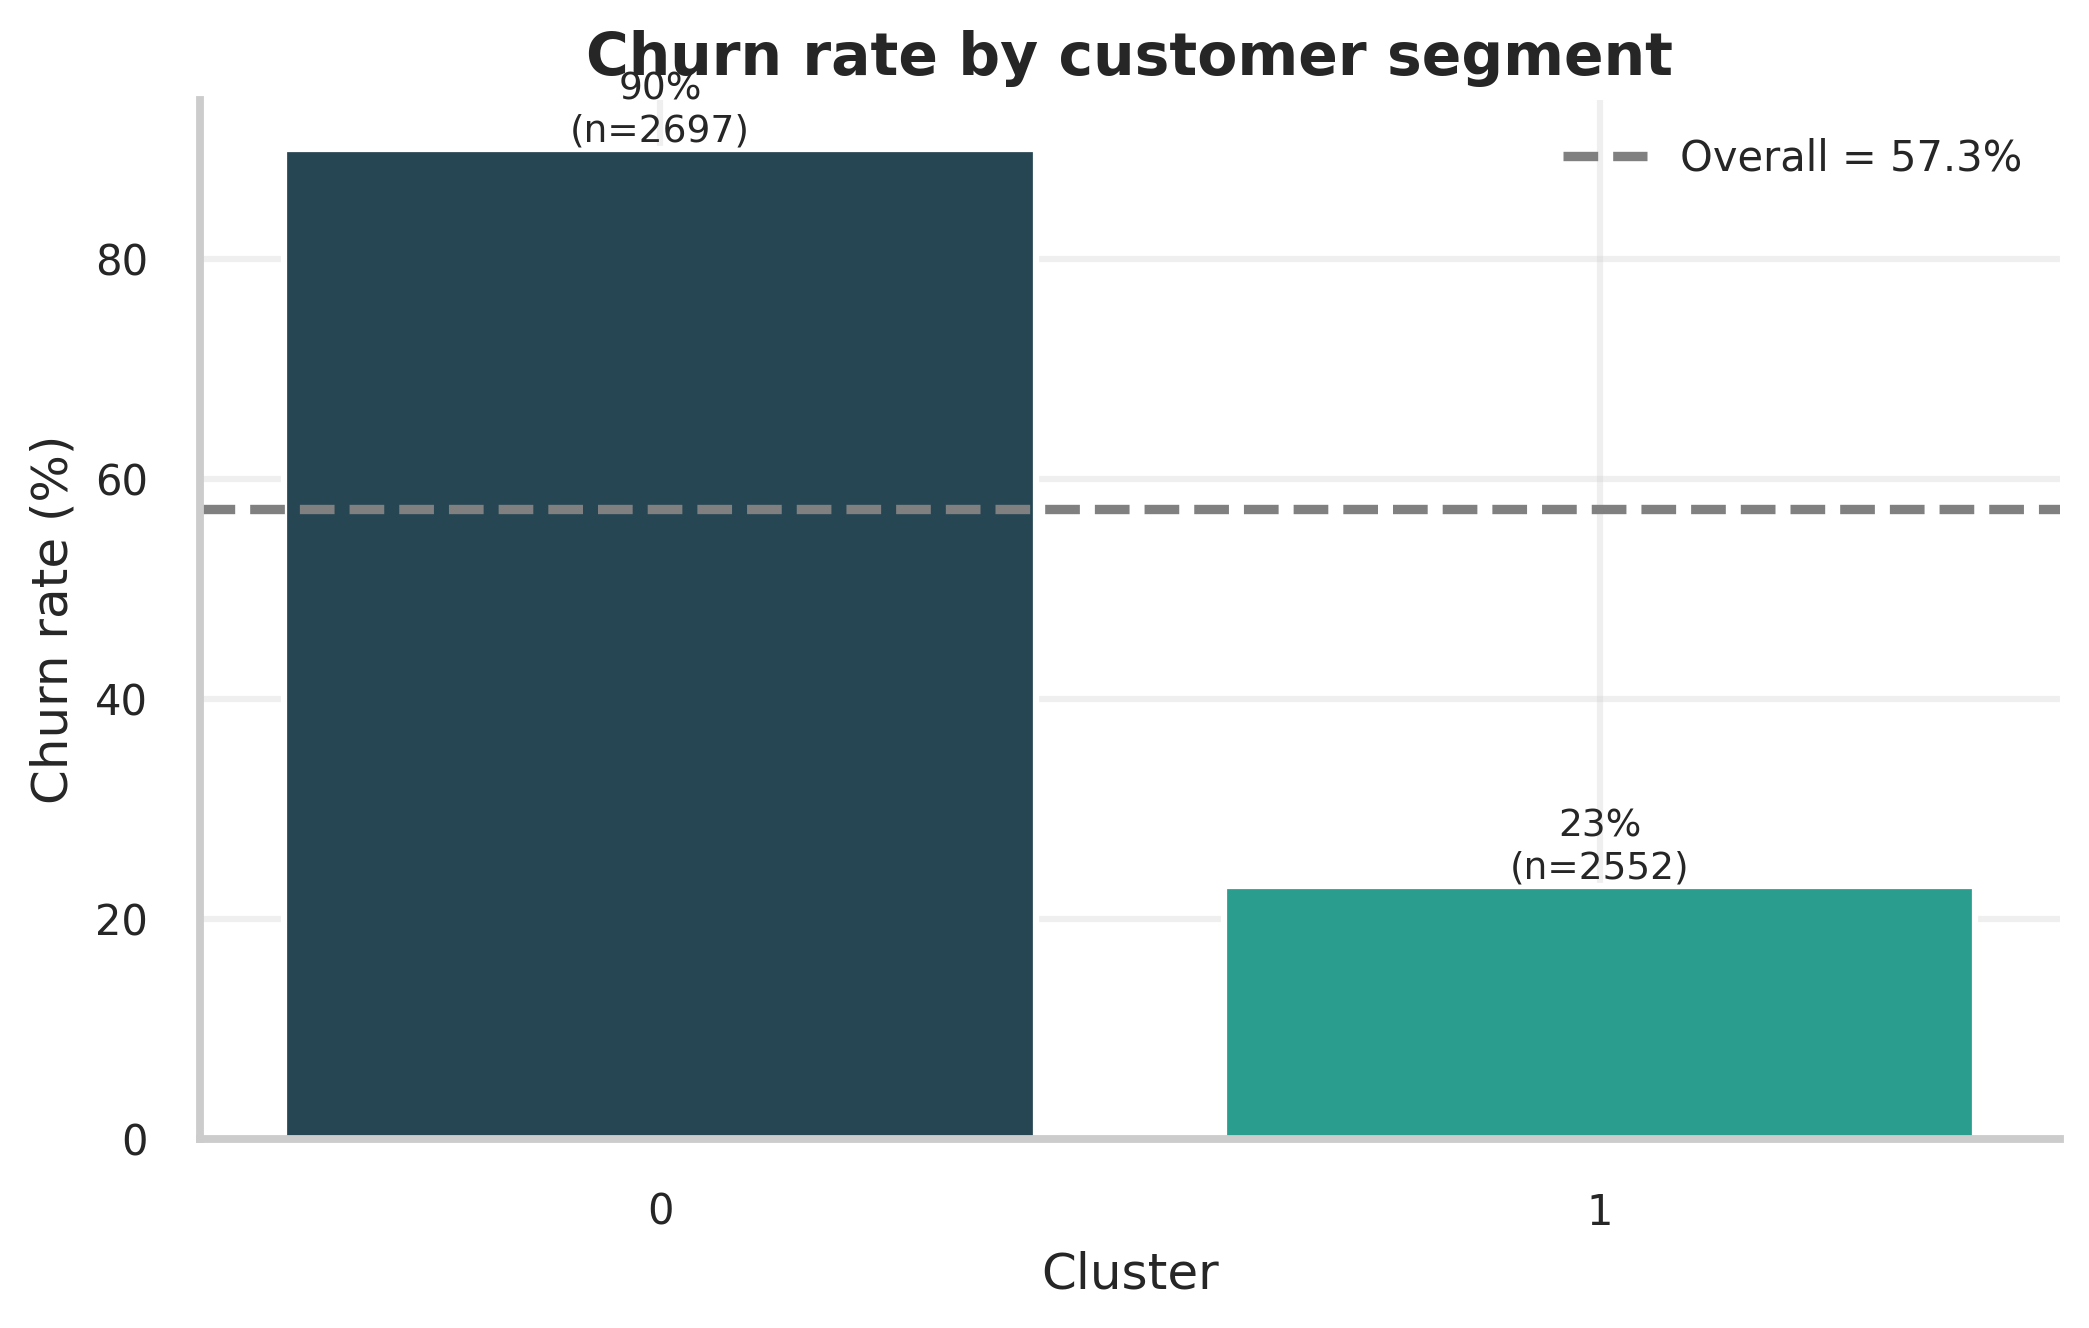
\includegraphics[width=\linewidth]{figures/06_churn_by_cluster.png}
  \caption{Churn rate by K-means segment; dashed line is the overall 57.4\% baseline. The {{churn_gap_points}}-percentage-point gap motivates segment-aware retention.}
  \label{fig:synth}
\end{figure}

\begin{figure*}[t]
  \centering
  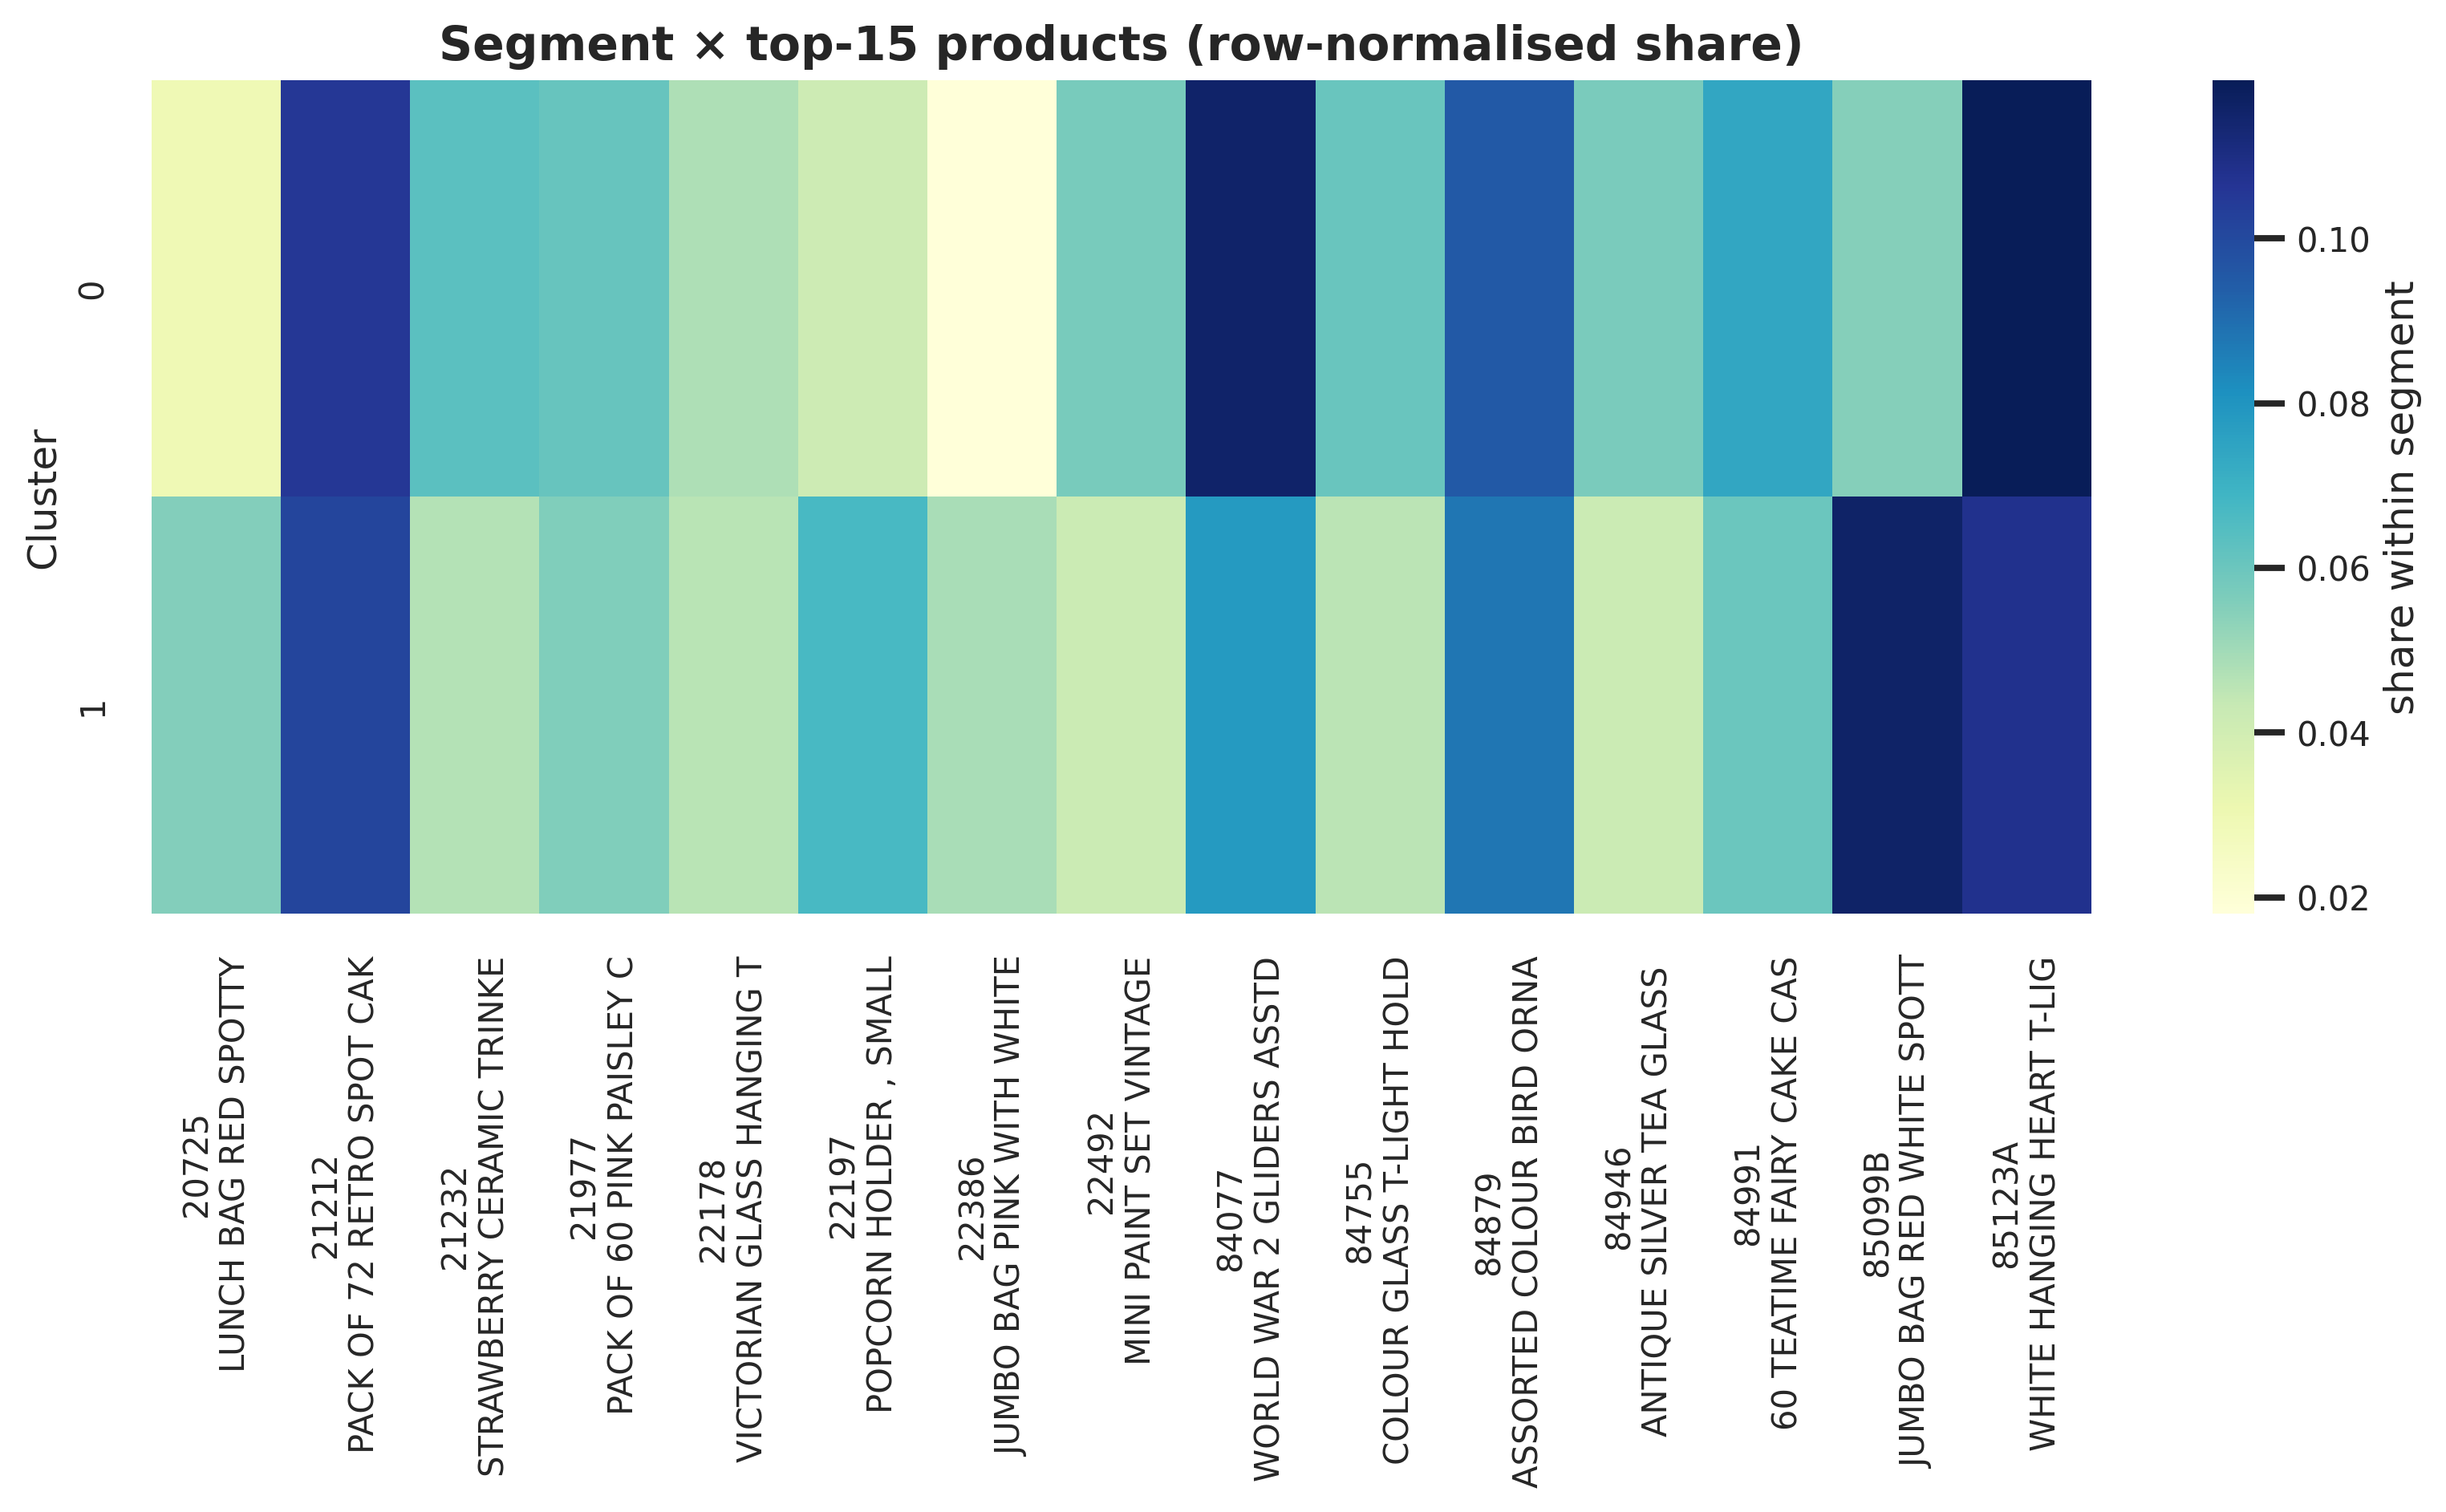
\includegraphics[width=0.92\textwidth]{figures/06_segment_products_heatmap.png}
  \caption{Segment $\times$ top-product heatmap (row-normalised purchase share). The \textit{Active loyal} segment concentrates on colour-coordinated sets, motivating the colour-pair cross-sell recommendation; the \textit{Dormant} segment's baskets are sparse and diffuse.}
  \label{fig:heatmap}
\end{figure*}

% ========================================================================
\section{Discussion and Limitations}
% ========================================================================
\textbf{Per-task winners.} For segmentation, K-means with $k=2$ dominates DBSCAN (which fragments badly under the heavy-tailed RFM distribution even after log-transform) and slightly edges AGNES on Silhouette and Calinski--Harabasz. For classification, {{classification_best_model}} and the tree ensembles cluster within roughly 0.03 AUC of one another and of the MLP ({{classification_mlp_auc}}), indicating that the RFM and behavioural feature set imposes a performance ceiling that additional model capacity does not break; the simpler, interpretable linear model is therefore preferred operationally. For association mining, FP-Growth's 1.5$\times$ runtime advantage over Apriori reproduces the well-known result at our problem size; the gap would widen at lower support thresholds.

\textbf{Limitations.} (i) Recency at the cutoff is strongly associated with the post-cutoff churn definition. To prevent this from leaking into the model we compute every supervised feature strictly before the cutoff and fit all transformers on training folds only, which brings the best AUC down from an inflated $\sim$0.99 (obtained with full-history features) to a realistic {{classification_best_auc}}. Honest baselines (majority {{majority_auc}}, recency-only {{recency_auc}}) and an ablation that removes Recency (AUC {{without_recency_auc}}) confirm the model still adds signal beyond Recency alone, and the predicted probabilities are well calibrated (Brier {{calibration_brier}}). (ii) The dataset is a single UK-centric retailer over two years with no demographic attributes, limiting generalisability and the depth of segment narratives. (iii) Cluster-specific association mining returned no rules for the dormant segment at our thresholds because dormant customers, by definition, have sparse invoices; lower support thresholds were tried but produced noisy long-tail rules. (iv) The autoencoder anomaly threshold is purely percentile-based; a domain-validated threshold would require labelled fraud or VIP outcomes which we do not have.

\textbf{Future work.} Promising directions include (i) sequence-aware DL such as Transformer-based purchase-sequence models that can predict next-basket as well as churn, (ii) uplift modelling to identify customers whose churn probability is most reducible by a retention offer (rather than those most likely to churn), and (iii) cross-retailer transfer to test whether the segment-aware retention rule generalises beyond a single store.

% ========================================================================
\section{Conclusion}
% ========================================================================
We presented a single end-to-end data mining pipeline on Online Retail II that simultaneously delivers customer segmentation (K-means $k=2$, Silhouette {{clustering_silhouette}}), leakage-safe 90-day churn prediction ({{classification_best_model}} AUC {{classification_best_auc}}; MLP AUC {{classification_mlp_auc}}, benchmarked against honest baselines), and market-basket pattern mining ({{association_n_rules}} association rules, top lift {{top_rule_lift}} via FP-Growth at 1.5$\times$ Apriori speed). Beyond reporting per-task results, the cross-task synthesis exposes a {{churn_gap_points}}-percentage-point churn gap between the dormant and active-loyal segments and shows that the loyal segment buys in color-coordinated pairs, producing the actionable recommendation to target loyal-segment churners with color-pair bundles. None of these recommendations is visible to any single model alone, which we take as evidence that integrating segmentation, classification, and association mining within one pipeline yields business insight greater than the sum of its parts.

% ========================================================================
\section*{Source code and dataset}
Source code, notebooks, and figures are submitted with this project package. Dataset: UCI Online Retail II \cite{uci_retail2}, \url{https://archive.ics.uci.edu/dataset/502/online+retail+ii}.

\bibliographystyle{IEEEtran}
\bibliography{references}

\end{document}
